%%%%%%%%%%%%%%%%%%%%%%%%%%%%%%%%%%%%%%%%%
% Journal Article
% LaTeX Template
% Version 1.4 (15/5/16)
%
% This template has been downloaded from:
% http://www.LaTeXTemplates.com
%
% Original author:
% Frits Wenneker (http://www.howtotex.com) with extensive modifications by
% Vel (vel@LaTeXTemplates.com)
%
% License:
% CC BY-NC-SA 3.0 (http://creativecommons.org/licenses/by-nc-sa/3.0/)
%
%%%%%%%%%%%%%%%%%%%%%%%%%%%%%%%%%%%%%%%%%

%----------------------------------------------------------------------------------------
%	PACKAGES AND OTHER DOCUMENT CONFIGURATIONS
%----------------------------------------------------------------------------------------

\documentclass[twoside,twocolumn,12pt]{article}

\usepackage{blindtext} % Package to generate dummy text throughout this template 

\usepackage[sc]{mathpazo} % Use the Palatino font
\usepackage[T1]{fontenc} % Use 8-bit encoding that has 256 glyphs
\linespread{1.5} % Line spacing - Palatino needs more space between lines
\usepackage{microtype} % Slightly tweak font spacing for aesthetics

\usepackage[english]{babel} % Language hyphenation and typographical rules

\usepackage[hmarginratio=1:1,top=25mm,columnsep=20pt,left=25mm]{geometry} % Document margins
\usepackage[hang, small,labelfont=bf,up,textfont=it,up]{caption} % Custom captions under/above floats in tables or figures
\usepackage{booktabs} % Horizontal rules in tables

\usepackage{lettrine} % The lettrine is the first enlarged letter at the beginning of the text

\usepackage{enumitem} % Customized lists
\setlist[itemize]{noitemsep} % Make itemize lists more compact

\usepackage{abstract} % Allows abstract customization
\renewcommand{\abstractnamefont}{\normalfont\bfseries} % Set the "Abstract" text to bold
\renewcommand{\abstracttextfont}{\normalfont\small\itshape} % Set the abstract itself to small italic text

\usepackage{titlesec} % Allows customization of titles
\renewcommand\thesection{\Roman{section}} % Roman numerals for the sections
\renewcommand\thesubsection{\roman{subsection}} % roman numerals for subsections
\titleformat{\section}[block]{\large\scshape\centering}{\thesection.}{1em}{} % Change the look of the section titles
\titleformat{\subsection}[block]{\large}{\thesubsection.}{1em}{} % Change the look of the section titles

\usepackage{fancyhdr} % Headers and footers
\pagestyle{fancy} % All pages have headers and footers
\fancyhead{} % Blank out the default header
\fancyfoot{} % Blank out the default footer
\fancyhead[C]{5584F $\bullet$ May 2020 $\bullet$ Harvey Hughes} % Custom header text
\fancyfoot[RO,LE]{\thepage} % Custom footer text

\usepackage{titling} % Customizing the title section

\usepackage{hyperref} % For hyperlinks in the PDF

\usepackage{graphicx}
\graphicspath{ {images/} }

\newenvironment{reusefigure}[2][htbp]
  {\addtocounter{figure}{-1}%
   \renewcommand{\theHfigure}{dupe-fig}% If you're using hyperref
   \renewcommand{\thefigure}{\ref{#2}}% Figure counter is \ref
   \renewcommand{\addcontentsline}[3]{}% Avoid placing figure in LoF
   \begin{figure}[#1]}
  {\end{figure}}
\usepackage{wrapfig}
\usepackage{amsmath}
\usepackage{xcolor}
\usepackage{listings}
\usepackage{subcaption}
\usepackage{pdfpages}
\usepackage{array,multirow,graphicx}
\lstset{
  basicstyle=\ttfamily,
  columns=fullflexible,
  frame=single,
  breaklines=true,
  postbreak=\mbox{\textcolor{red}{$\hookrightarrow$}\space},
}

\newcommand{\threepartdef}[6]
{
	\left\{
		\begin{array}{lll}
			#1 & \mbox{: } #2 \\
			#3 & \mbox{: } #4 \\
			#5 & \mbox{: } #6 \\
			0 & \mbox{: } otherwise
		\end{array}
	\right.
}
\usepackage{multicol}
\usepackage{stfloats}

%----------------------------------------------------------------------------------------
%	TITLE SECTION
%----------------------------------------------------------------------------------------

\setlength{\droptitle}{-4\baselineskip} % Move the title up

\pretitle{\begin{center}\Huge\bfseries} % Article title formatting
\posttitle{\end{center}} % Article title closing formatting
\title{Robotic Unicycle} % Article title
\author{%
\textsc{Final Report} \\
\\
\textsc{Harvey Hughes} \\
\textsc{Supervisor:Professor Carl Rasmussen} \\
}
\date{\today} % Leave empty to omit a date
\renewcommand{\maketitlehookd}{%

}

%----------------------------------------------------------------------------------------

\begin{document}

% Print the title
\maketitle

%----------------------------------------------------------------------------------------
%	ARTICLE CONTENTS

\section*{Technical Abstract}
The application of machine learning to calculate a control policy opposed to using control theory could prove to be highly useful when its not possible to determine system dynamics. However, success outside of simulations has been slow. A robotic unicycle is considered in this project with tests into roll limit, sampling time, phone connection and initial orientation being tested first in order to brooch the gap between simulation and real success.

\clearpage
a
\onecolumn

%----------------------------------------------------------------------------------------
\tableofcontents

\twocolumn

\begin{figure*}[b!]
  \centering
  \begin{subfigure}[t]{0.325\textwidth}
    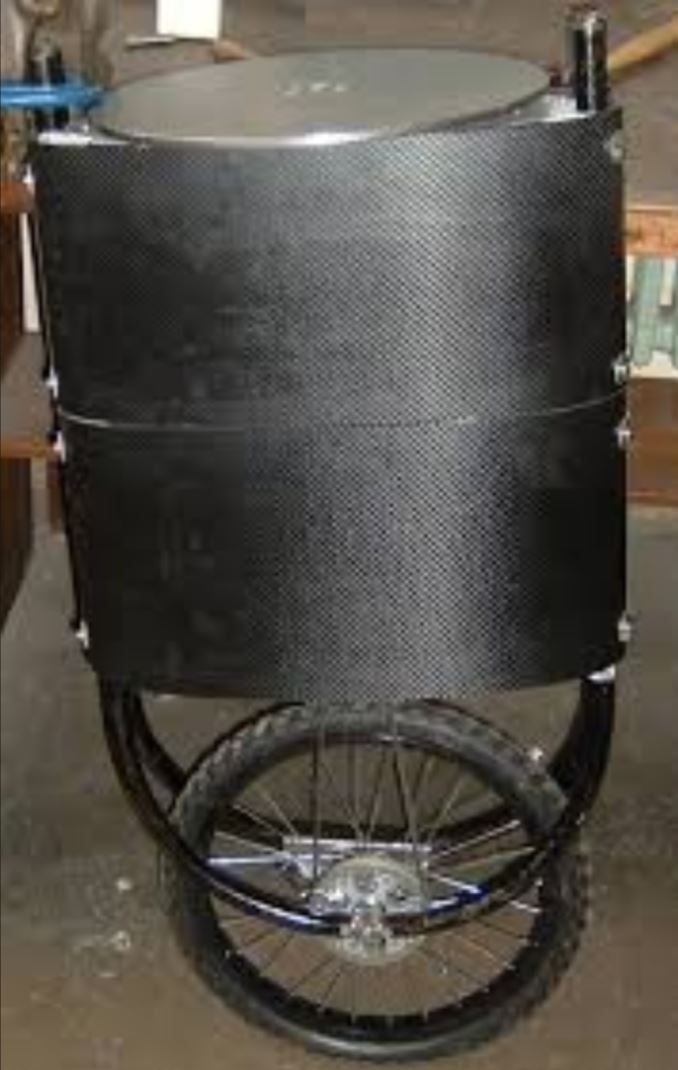
\includegraphics[width=\linewidth,height=7.5cm]{first}
   \caption{1m tall 1st model \cite{roderigo}}
  \label{sub:old1}
  \end{subfigure}
  \begin{subfigure}[t]{0.325\textwidth}
    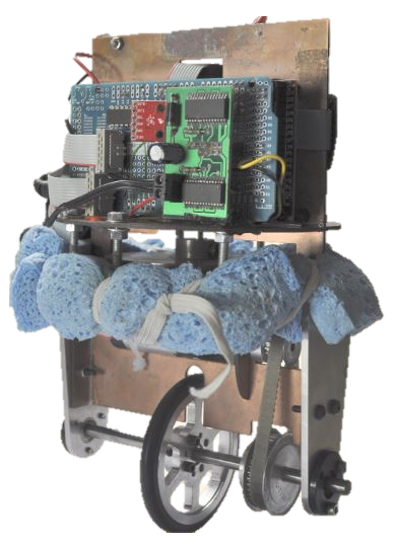
\includegraphics[width=\linewidth,height=7.5cm]{old_unicycle}
    \caption{20cm tall 2nd model \cite{eric}}
  \label{sub:old2}
  \end{subfigure}
  \caption{Previous unicycle iterations}
  \label{fig:unimodels}
\end{figure*}
\section{Introduction}
\subsection{Project aims}
\lettrine[nindent=0em,lines=3]{T}he aim of this project is to create a controller that is able to balance a robotic unicycle. The controller starts off with no information about the system, and is therefore required to slowly learn what are good actions to make. This mimics the way in which humans learn new tasks as children by trying new actions and seeing if they're beneficial.
\newline
This is an ongoing project from previous years where success has been shown in simulations yet has so far been hard to achieve in real life. A major outcome of this project is the build upon previous years work and fix existing issues, in addition to solving new ones in order to bring the success of a real unicycle closer to simulations. 
\newline
This project aims to demonstrate the effectiveness of implementing the PILCO algorithm \cite{pilco} on more complex dynamic systems. PILCO has previously been shown to tackle simpler problems such as a cart-pole system with less data and high speeds compared to other algorithms. 
\newline 
A unicycle is a suitable example to test on due to the complex nature of the problem, even for human riders. Balancing on the spot is additionally a less linear and therefore harder problem to solve then simply moving forward. This complexity allows the full extremes of the PILCO algorithm to be explored and therefore demonstrate all flaws and benefits in PILCO.
%---------------------------





\subsection{Previous work}
Work has been conducted on robotic unicycles within the engineering Department on and off since 2005 \cite{original}. This unicycle was full sized at 1m, and weighed 35kg shown in figure \ref{sub:old1}. Built by Mellors and Lamb the unicycle involved a wheel motor and horizontal flywheel motor to mimic the rotation arms can create. Having the flywheel in the horizontal plane increases the complexity over other designs with in in the vertical plane, as it couples the two motors together when a roll angle is corrected.
\newline
The problem was originally being solved using control theory approaches. This involved complex analysis of the dynamics in 2D and 3D conducted in 2007-2009 by D'Souza-Mathew \cite{neil} and Forster  \cite{forster}. Some success was demonstrated at balancing the unicycle. However, simplifications in the analysis resulted in non-linearities present in real life to not be considered accurately.
\newline
In 2010 Mchutchon \cite{mchut} applied the RMLC (Reinforced Model Learnt Control) algorithm developed by Rasmussen and Deisenroth to the unicycle, and acived balancing of a unicycle with stabilisers. In 2011 building upon Mchutcons work Queiro \cite{roderigo} and Douglass \cite{douglass} were able to modify the unicycle to balance unrestrained for up to 5 seconds. 
\newline
The size of the unicycle posed serious safety risks, both in terms of replacing large components and the need to limit the unicycle during tests. One way this was done was by attaching to bike racks \cite{neil} or suspending the unicycle from the department atrium \cite{roderigo}. These methods while reducing the risk didn't eliminate it, and caused unnecessary simplifications or disturbances to the unicycle dynamics. 
\newline
To increase safety a small model unicycle was constructed as in figure \ref{sub:old2}. PILCO was also implemented on the unicycle \cite{pilco}. The increased safety of the smaller unicycle allowed unconstrained motion to be tested more easily. Work began on the miniature unicycle in 2015 by Tukiainen \cite{tuk}. Problems in balancing the unicycle were encountered at this point, with concerns about identifying the cause for problems. In 2017 an overhaul of the software was done by Wieser \cite{eric}, and in 2019 an electrical overhaul by Harris \cite{arsalan}. This was to simplify the system and allow for more accurate troubleshooting. 

\begin{figure*}[t!]
  \centering
  \begin{subfigure}[t]{0.325\textwidth}
    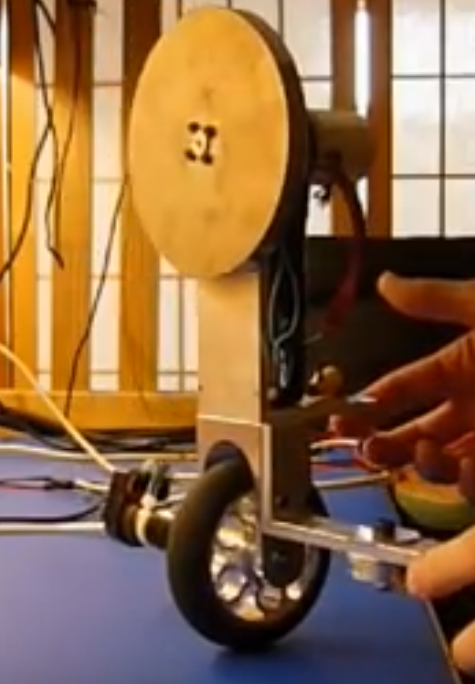
\includegraphics[width=\linewidth,height=7.5cm]{other1}
   \caption{\cite{other1}}
  \label{sub:oother1}
  \end{subfigure}
  \begin{subfigure}[t]{0.325\textwidth}
    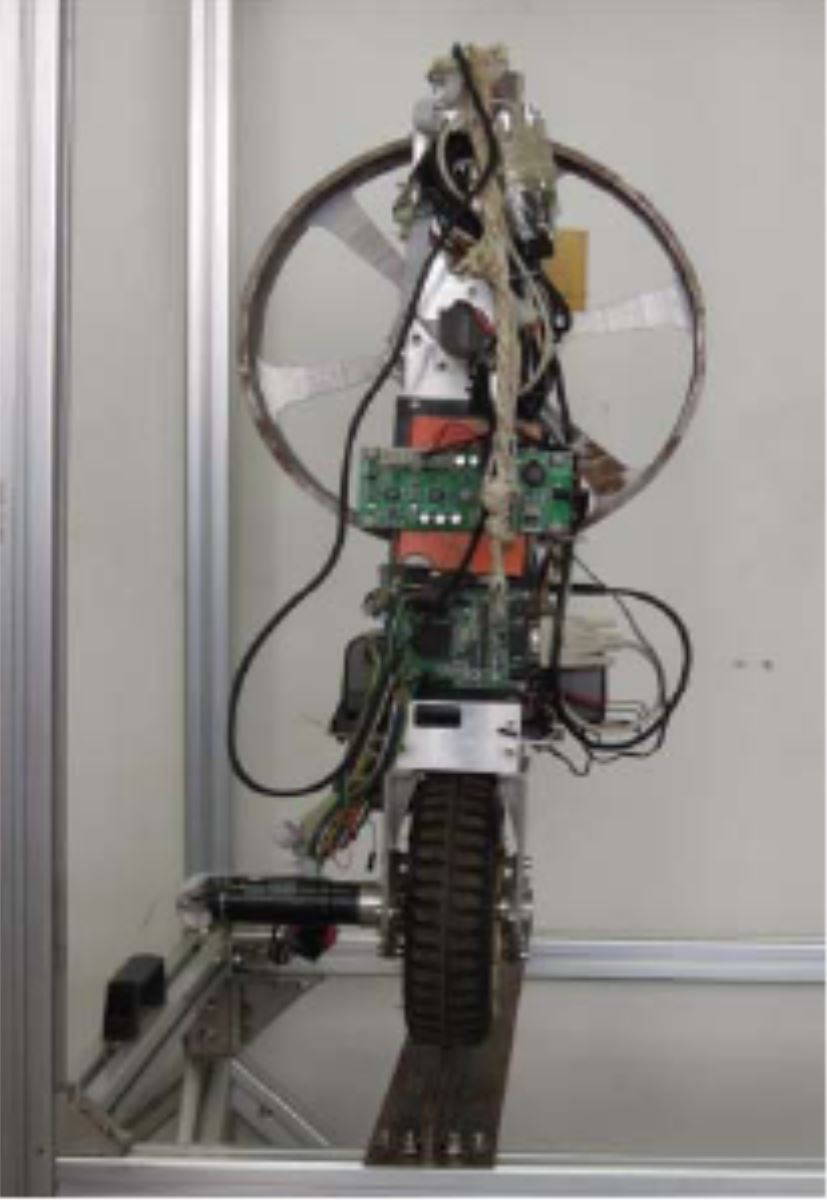
\includegraphics[width=\linewidth,height=7.5cm]{other3}
    \caption{\cite{other2}}
  \label{sub:other2}
  \end{subfigure}
  \caption{Other Unicycle designs}
  \label{fig:otheruni}
\end{figure*}

%---------------------------
\subsection{Examples of other unicycles}
There are numerous examples of other work conducted on balancing robotic unicycles. Many of these involved a large vertical flywheel and use of control theory as seen in figure \ref{fig:otheruni}. Orientating the disk this way improves stability and was therefore quite successful at balancing. The improved stability is due to uncoupling the two torques, meaning that to correct a roll error just the flywheel can be used, and to correct a pitch error the wheel only needs rotating. A combination of both actions is required to fix roll errors on a unicycle with horizontal flywheel.



There has been work done on unicycles set-up with a horizontal flywheel. \cite{other3}. Vos and Von Flotow analysed a large unicycle and were able to balance to some success. This required multi region control policies to work, and therefore was very complicated.
\newline
The robotic unicycles discussed so far have all been developed using traditional control theory. Very few unicycles have been controlled with a machine learning approach. Simulations of a 2D unicycles were successfully balanced \cite{other4} using standard keras and Tensorflow libraries. However, this approach simplifies the problem back to a much easier inverted pendulum, and didn't deal with the problems associated with real models. The lack of previous success at this particular task highlights its difficulty.

%------------------------------------------------
\clearpage
\section{Theory}
\subsection{Coordinate System}
In order to fully define the unicycle state at each time step seven coordinates and their derivatives are required. These coordinates are shown in figure \ref{fig:ang} giving the state as

\begin{align*}
\textbf{x} = [\dot{x} \: \dot{y}\: \dot{\theta}\: \dot{\phi}\: \dot{\psi}_f\: \dot{\psi}_w \:\dot{\psi}_t \: x \: y \: \theta \: \phi \: \psi_f \: \psi_w \: \psi_t]^T
\end{align*}


\begin{figure}[h]
  \centering
  \begin{subfigure}[t]{0.1935\textwidth}
    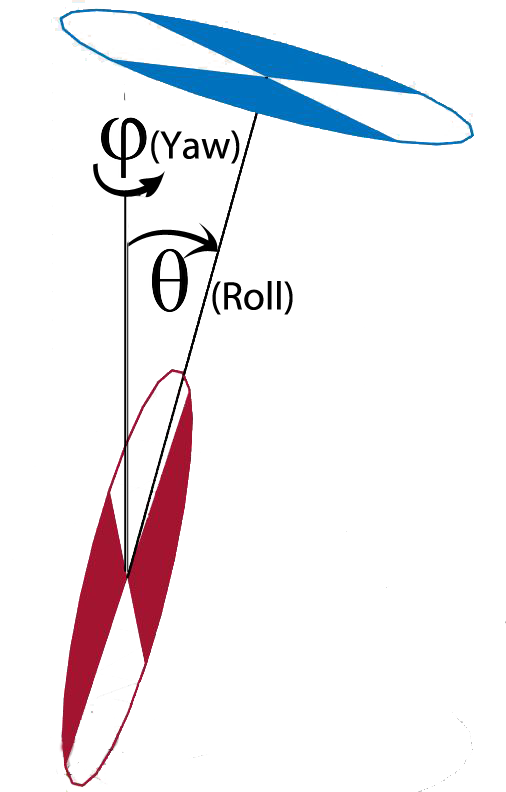
\includegraphics[width=\linewidth]{end_labled2}
  \label{fig:e}
  \end{subfigure}
  \begin{subfigure}[t]{0.2295\textwidth}
    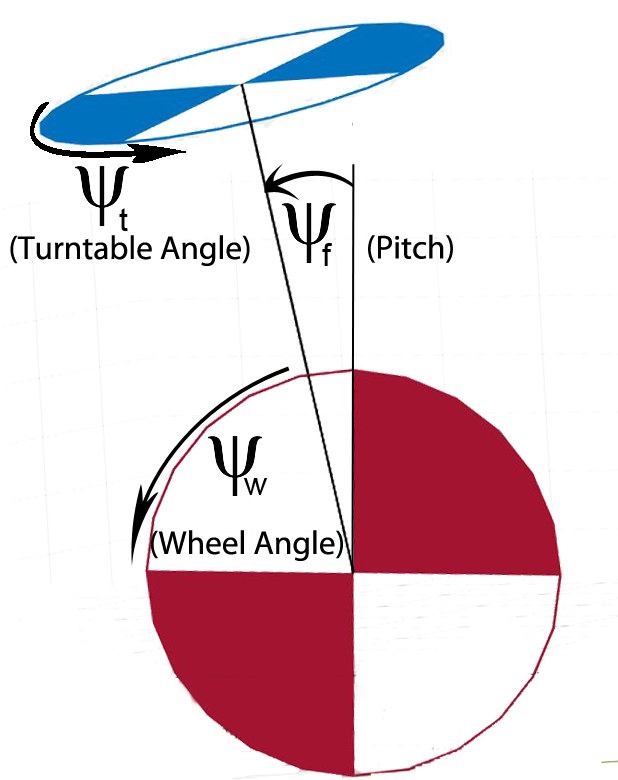
\includegraphics[width=\linewidth]{side_labled}
  \label{fig:s}
  \end{subfigure}
  \caption{Angles used to define position}
  \label{fig:ang}
\end{figure}

In order to define rotations in 3D to represent $\theta,\phi,\psi_f$ correctly care must be taken to the order the rotations are applied. This is because rotations are non commutative in 3D unlike in 2D. The convention of Euler angles is used to solve this problem. \cite{eric}
\newline
There are 12 orders of rotation which can be used. XYZ or 123 convention is used on the unicycle as in equation \ref{eq:eul}. Where $R_A(\alpha)$ represents a right hand rotation about axis A of $\alpha$. 

\begin{equation}
R_{XYZ}(\psi_f,\theta,\phi)\textbf{x} = R_X(\psi_f)R_Y(\theta)R_Z(\phi)\textbf{x}
\label{eq:eul}
\end{equation}

%-------------------------------
\subsection{Quaternions}
As discussed previously rotations in 3D are difficult to combine due to their non-commutative nature. A handy way of dealing with consecutive rotations is to use quaternions. These are an extension of complex numbers to include three imaginary parts and are written as:

\begin{align*}
a + b\textbf{i} + c\textbf{j} + d\textbf{k}
\end{align*}

The following properties allow quaternions obey the same rules as 3D rotations:

\begin{align*}
\textbf{i}^2 = \textbf{j}^2 = \textbf{k}^2 = \textbf{ijk} = -1
\end{align*}

A rotation about axis (x,y,z) by $\alpha$ can be defined using the following unit quaternion \cite{quat}

\begin{gather}
\textbf{q}_{rot} = cos(\frac{\alpha}{2}) + sin(\frac{\alpha}{2})x\textbf{i} + sin(\frac{\alpha}{2})y\textbf{j} + sin(\frac{\alpha}{2})z\textbf{j} \nonumber \\
\textbf{q}_{new} = \textbf{q}_{old} . \textbf{q}_{rot} \nonumber
\end{gather}

%----------------------------------
\subsection{Optimal Control}
 
 
%--------------------------------------------------------

\subsection{PILCO}
In policy optimisation an algorithm called PILCO \cite{pilco} will be used.
This method will optimise a policy to decide the best action $\textbf{u}$ given the unicycles state. To determine optimum actions the expected loss over a horizon is evaluated under the current policy, as in equation \ref{eq:pilco}.


\begin{equation}
\begin{split}
\pi^*(\textbf{x}) = argmin \sum_0^tc(\textbf{x}^{(i)}) \\
\textbf{u}^{(i)} = \pi(\textbf{x}^{(i)} )\\
\end{split}
\label{eq:pilco}
\end{equation}


%-----------------------------------
\subsection{Gaussian Processes}

A Gaussian process is used to model the dynamics and gives a range of possible functions which fit observed data in a non parametric way as to not introduce model bias. A Gaussian process is a generalisation of a multivariate Gaussian to infinitely many variables. As a result a mean and covariance function are used to define it as in equation \ref{eq:gp}.
\begin{equation}\label{eq:gp}
\begin{gathered}
f(\textbf{x}) \sim \mathcal{GP}(m(\textbf{x},k(\textbf{x},\textbf{x'})) \\
m(\textbf{x}) = \mathbb{E}[f(\textbf{x})]  \\
k(\textbf{x},\textbf{x'}) = \mathbb{E}[(f(\textbf{x})-m(\textbf{x}))( f(\textbf{x'})-m(\textbf{x'}))]
\end{gathered}
\end{equation}

A major advantage of PILCO is the ability to retain uncertainty throughout this process. This means an initial state distribution can be propagated forward to generate a state distribution at each time step. These distributions are used to calculate the average instantaneous cost in policy evaluation.
The uncertainty grows over time and comes from an initial variation in start position, measurement noise, and process noise. 

\begin{figure}[h]
  \centering
  \begin{subfigure}[t]{0.5\textwidth}
    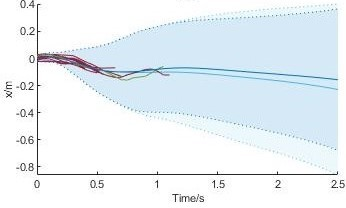
\includegraphics[width=\linewidth]{u2}
  \caption{x Prediction} 
  \label{sub:ffffffs}
  \end{subfigure}
  \begin{subfigure}[t]{0.5\textwidth}
    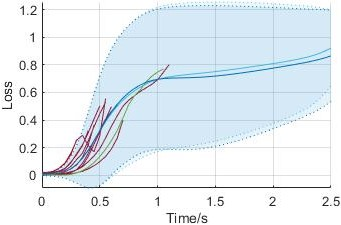
\includegraphics[width=\linewidth]{loss2}
  \caption{Loss prediction}
  \label{sub:ffs}
  \end{subfigure}
  \caption{Predictions from PILCO approach}
  \label{fig:pilco}
\end{figure}

Figure \ref{sub:ffffffs} shows predicted x position, with predictions up to 0.5s showing low uncertainty. After this the model loses the ability to predict the state accurately and the state distribution widens. 
A similar trend is observed for the predicted loss at each time step in figure \ref{sub:ffs}.
\newline
PILCO uses an iterative approach to optimising policy. Initially a random controller is used to get sufficient data for a dynamic model. Policy optimisation and rollouts under the new policies can then occur until the task is either learnt or terminated. 


%---------------------------------------------------------------
\subsection{Cost Function}
A cost function is required to evaluate the performance at each timestep. This takes the form of equation \ref{eq:simple}. Where a, h and $\theta_{max}$ represent positive constants, and d(\textbf{x}) is the geometric distance of the unicycle tip from the starting position.


\begin{equation}
\label{eq:simple}
\begin{gathered}
c(\textbf{x}) = 1 - \mathcal{R}(\textbf{x}) \\ 
\mathcal{R}(\textbf{x}) = exp(-\frac{a}{2h^2}d(\textbf{x})^2 - \frac{\phi^2}{2(4\pi)^2} - \frac{\theta^2}{\theta_{max}^2}) 
\end{gathered} 
\end{equation}
%------------------------------------------

\clearpage

\begin{figure*}[t!]
  \centering
  \begin{subfigure}[t]{0.325\textwidth}
    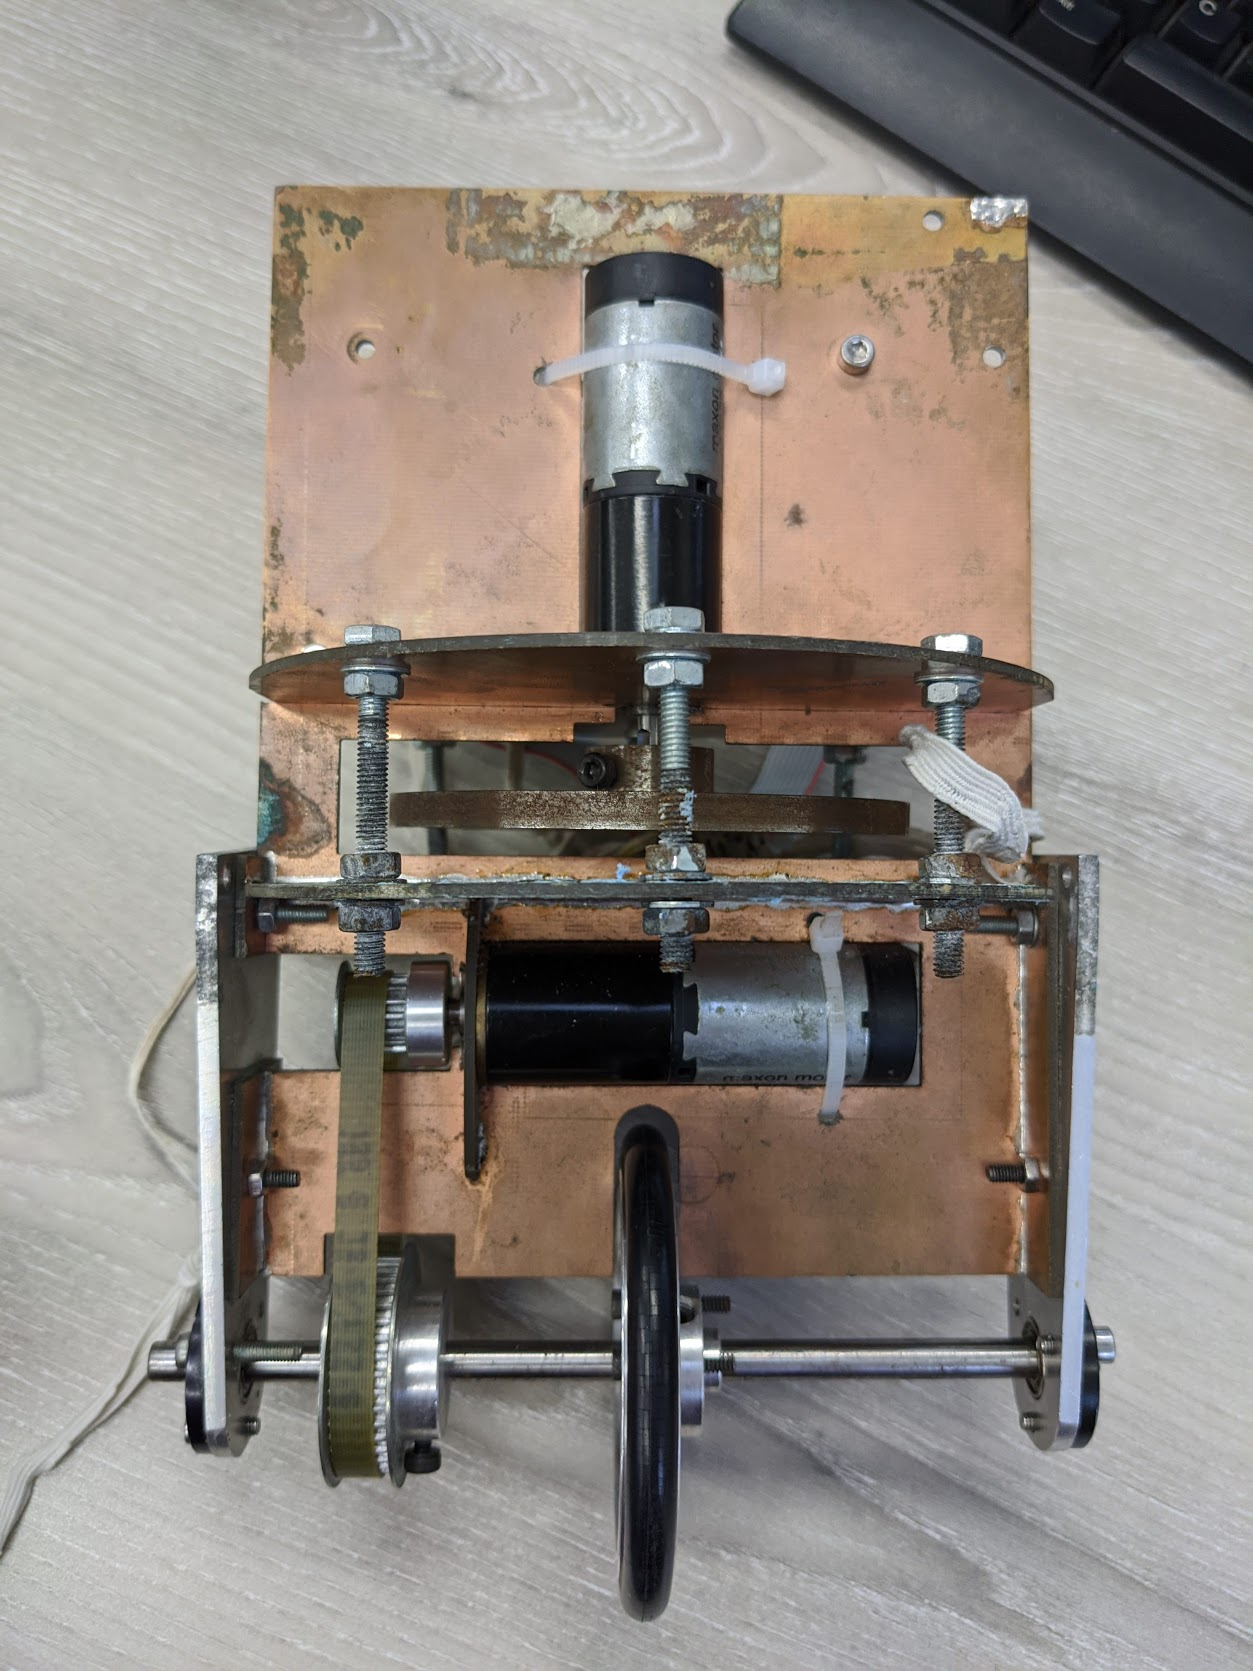
\includegraphics[width=\linewidth,height=7.5cm]{uni_old_mech}
   \caption{Frame}
  \label{sub:frameold}
  \end{subfigure}
  \begin{subfigure}[t]{0.325\textwidth}
    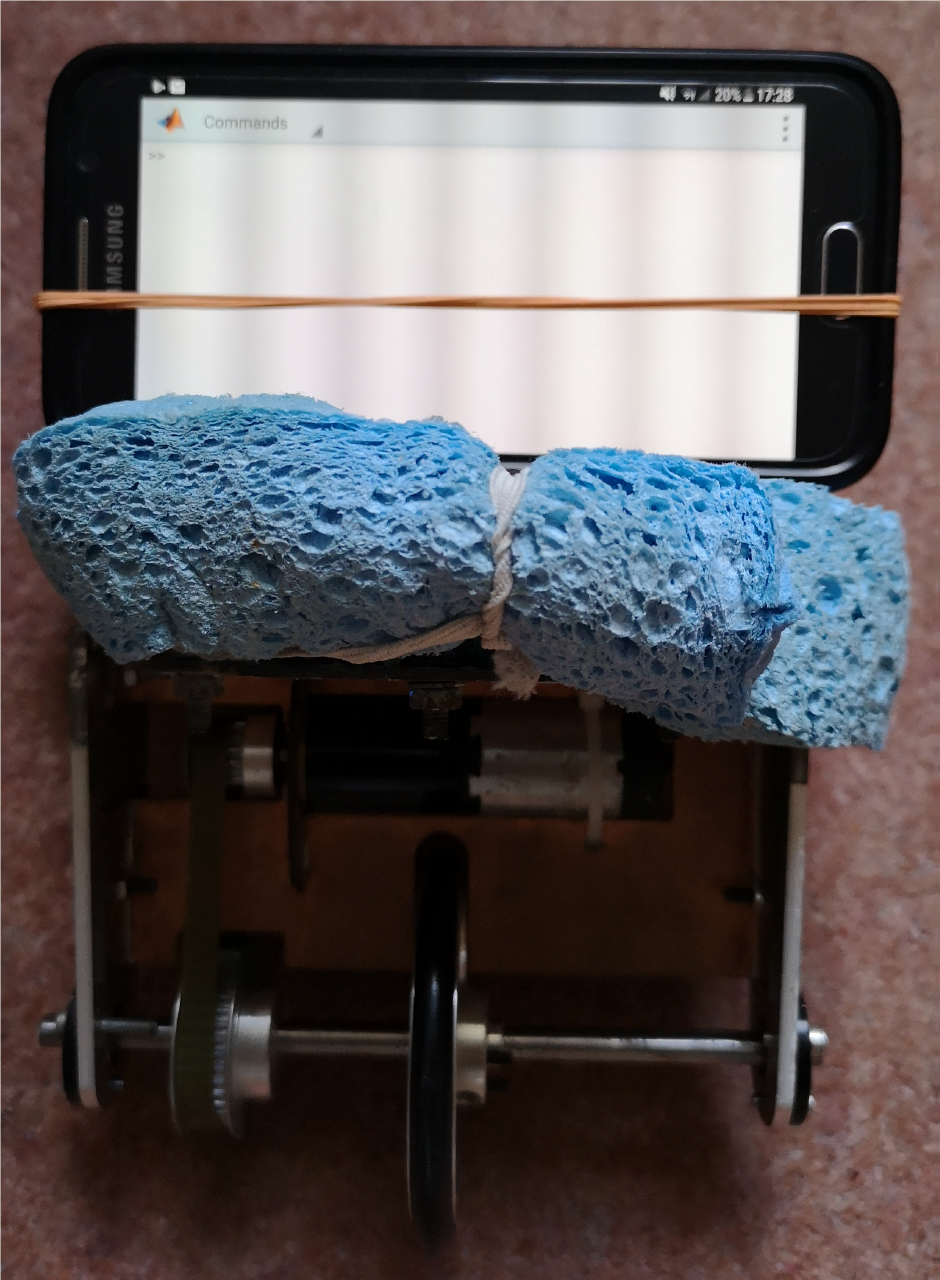
\includegraphics[width=\linewidth,height=7.5cm]{old1}
    \caption{Front \cite{arsalan}}
  \label{sub:frontold}
  \end{subfigure}
  \begin{subfigure}[t]{0.325\textwidth}
    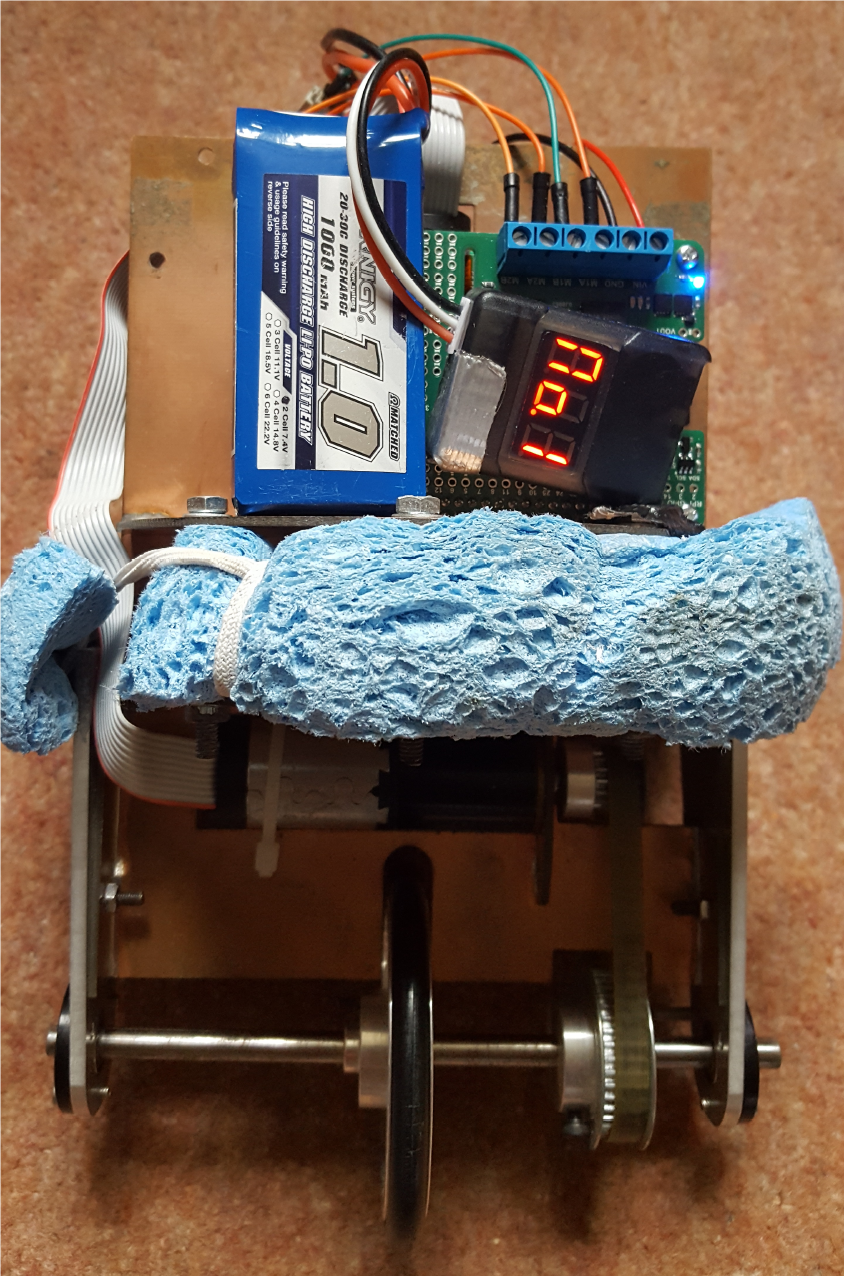
\includegraphics[width=\linewidth,height=7.5cm]{old2}
    \caption{Back \cite{arsalan}}
  \label{sub:backold}
  \end{subfigure}
  \caption{Current set-up of unicycle}
  \label{fig:current}
\end{figure*}


\section{Current Unicycle Set-up}


\subsection{Mechanical}



\subsection{Electrical}
\subsection{Software}

An Android phone is used as the gyroscope and accelerometer for reading the current state. The sensor data is transmitted from the phone to a computer running the policy script before the required action is transmitted to a raspberry pi to controls the motors.

%----------------------------------

\clearpage
\section{Initial Simulation Results}

During previous years the Unicycles performance on the real model was relatively poor. A mechanical redesign was considered to fix some of these issues. In order to evaluate the performance of this redesign and additional factors simulations were conducted as they allowed a quick and easy way to alter variables.
\newline

%-------------------------------
\subsection{Test Procedure}

Two different measures will be used to determine success. The first being time upright as more rollouts occur. This is to determine any success at balancing the model has. The second is total rollout loss in order to see if success is achieved by staying near the origin instead of staying upright.
%......................................................
\subsection{Roll Limit}
\begin{figure*}[ht!]
  \centering
  \begin{subfigure}[t]{0.325\textwidth}
    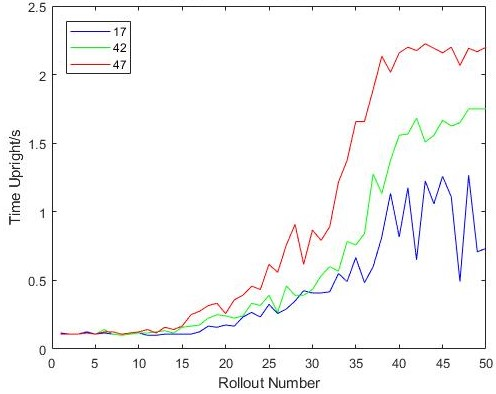
\includegraphics[width=\linewidth]{a2}
   \caption{Average of six tests}
  \label{fig:a}
  \end{subfigure}
  \begin{subfigure}[t]{0.325\textwidth}
    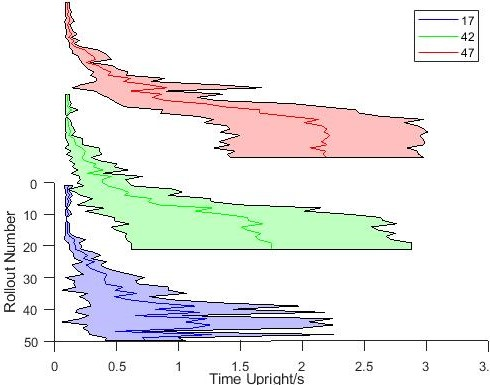
\includegraphics[width=\linewidth]{r2}
    \caption{With $\pm \sigma$}
  \label{fig:sd}
  \end{subfigure}
  \begin{subfigure}[t]{0.325\textwidth}
    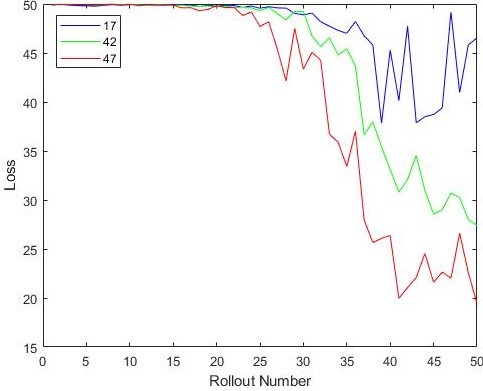
\includegraphics[width=\linewidth]{lossav}
    \caption{Comparing against rollout loss}
  \label{fig:rl}
  \end{subfigure}
  \caption{Simulating the effect of roll limit $\theta_{max}$ }
  \label{fig:rolllimit}
\end{figure*}
The first factor that would determine the benefit of a large mechanical redesign is the roll limit. In the unicycle model the roll angle cannot exceed 17 degrees. This is thought to inhibit learning as initially the system can't balance and will hit this limit within very few time steps. This could mean the model has insufficient data to successfully learn a policy. Futhermore as the last measurment is removed in real trials due to high accelerations the data available is reduced more. This reduction will have a larger effect on small roll limts and can cause failure to appear to happen at a low cost. Which could in turn inhibit learning more.
\newline
Several designs were sketched to change the roll limit. 42 degrees could be achieved with a new chassis and the same gears, and 47 degrees by changing an additional bracket. Simulations of these can be seen in figure \ref{fig:rolllimit}.
\newline
After 10 random rollouts the roll limit made little difference as in figure \ref{fig:a}. However, when policy optimisation started then a higher roll limit improved success greatly. The change between 42 and 47 degrees appears significant which shows more progress is likely to be made by increasing roll limit further. The plateau observed at 47 degress is due to some tests consistently staying upright for the whole horizon time. When looking at rollout total loss in figure \ref{fig:rl} the same pattern is observed with a higher roll limit reducing the overall rollout loss.
\newline
The variation between simulations can be seen in figure \ref{fig:sd} and shows greater reliability at higher roll limits, with a standard deviation of spread at 47 degrees close to being higher then the mean at 42 degrees. The spread is very important to create a reliable policy training method.
\newline
Higher roll limits could be achieved by changing other parts. 53 degrees would require a 5mm larger wheel. This change would require evaluating the effect wheel size had on performance as well as roll limit.

%-----------------------------------
\subsection{Sampling Time}
Sampling time is another important factor to consider when optimising the training situation of the real unicycle. A faster sampling time effects the following:

\begin{itemize}
\item Dynamics change slower and more linearly between readings, decreasing modelling complexity and improving predictions.
\item A zero order hold controller is used on the motors, with torque calculated at the start of a step. As the unicycle moves this action is non optimum, therefore an error is introduced.
\item More data points are collected, this can help build better models but at the expense extra computational time.
\item Every policy call injects noise into the predictions from process and measurement noise. This causes a more uncertain trajectory prediction over the horizon time.
\end{itemize}

Not enough tests have been simulated yet to fully determine the effect. However, new learning behaviours which prioritised distance to origin over just being upright were observed. Therefore showing promise that sampling time can greatly effect learning.

\begin{figure}[h]
  \centering
    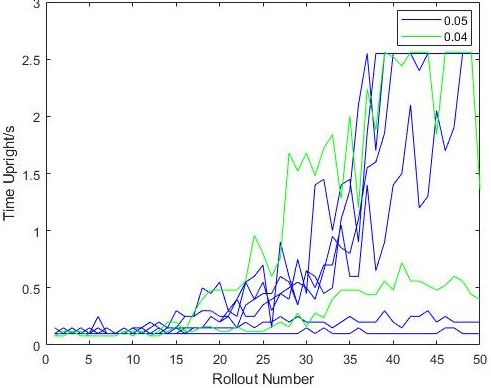
\includegraphics[width=\linewidth]{timestepeffect}
  \caption{Effect of sampling time change}
  \label{fig:st}
\end{figure}
Figure \ref{fig:st} shows the results of changing timestep for a roll limit of 42 degrees. Not enough tests have been conducted yet due to the increased simulation time meaning no conclusions can be drawn yet. The lower performing trial at 0.04s did show promise as it learnt to balance in a different way to all other trials, it prioritised staying at the origin over staying upright. This shows that there is a possibility of the timestep greatly effecting learning and should be pursued further.

%---------------------------------------------
\subsection{Wheel Size}

%--------------------------------
\subsection{Future Simulations}
Additional factors are to be simulated to determine the variables that effect learning rate the most. These are the following:

\begin{itemize}
\item Higher roll limits with larger wheels.
\item More sampling times.
\item Strength of the cost function.
\item Motor torques.
\end{itemize}
%------------------------------------------------


%---------------------------------------
\clearpage

\begin{figure*}[t!]
  \centering
  \begin{subfigure}[t]{0.325\textwidth}
    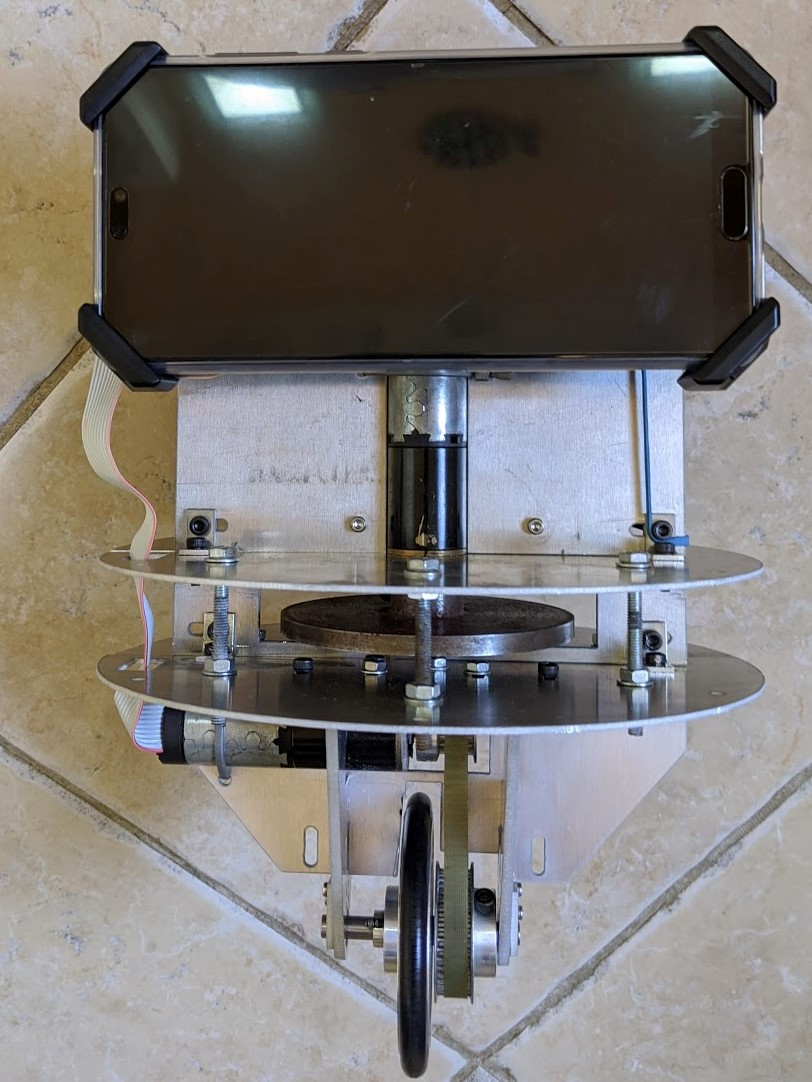
\includegraphics[width=\linewidth]{frontnew}
   \caption{Front}
  \label{sub:frontnew}
  \end{subfigure}
  \begin{subfigure}[t]{0.325\textwidth}
    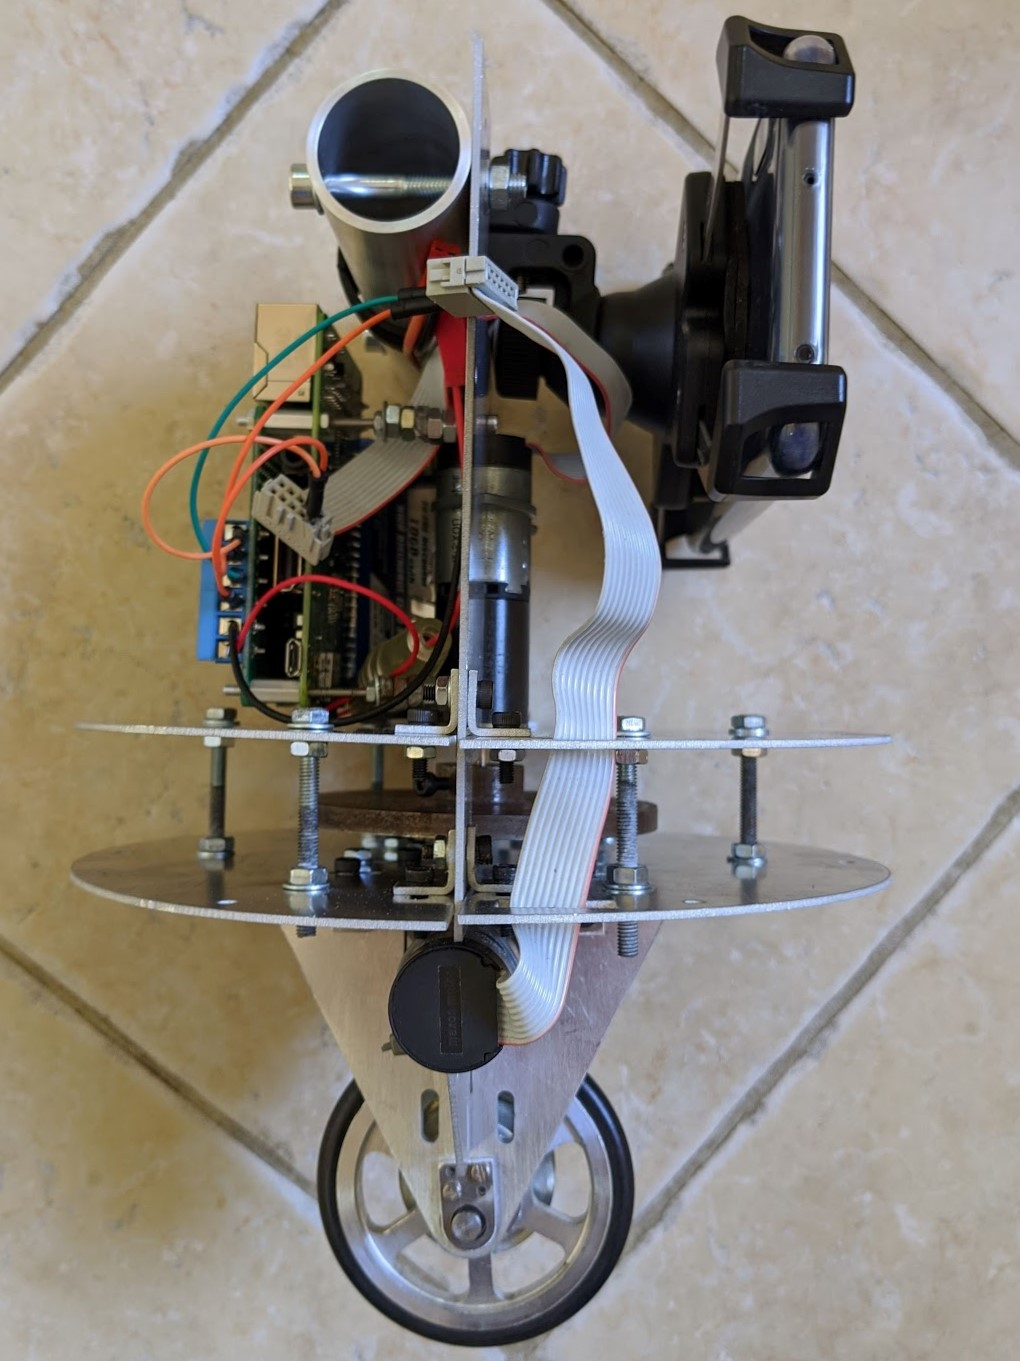
\includegraphics[width=\linewidth]{sidenew}
    \caption{Side}
  \label{sub:sidenew}
  \end{subfigure}
  \begin{subfigure}[t]{0.325\textwidth}
    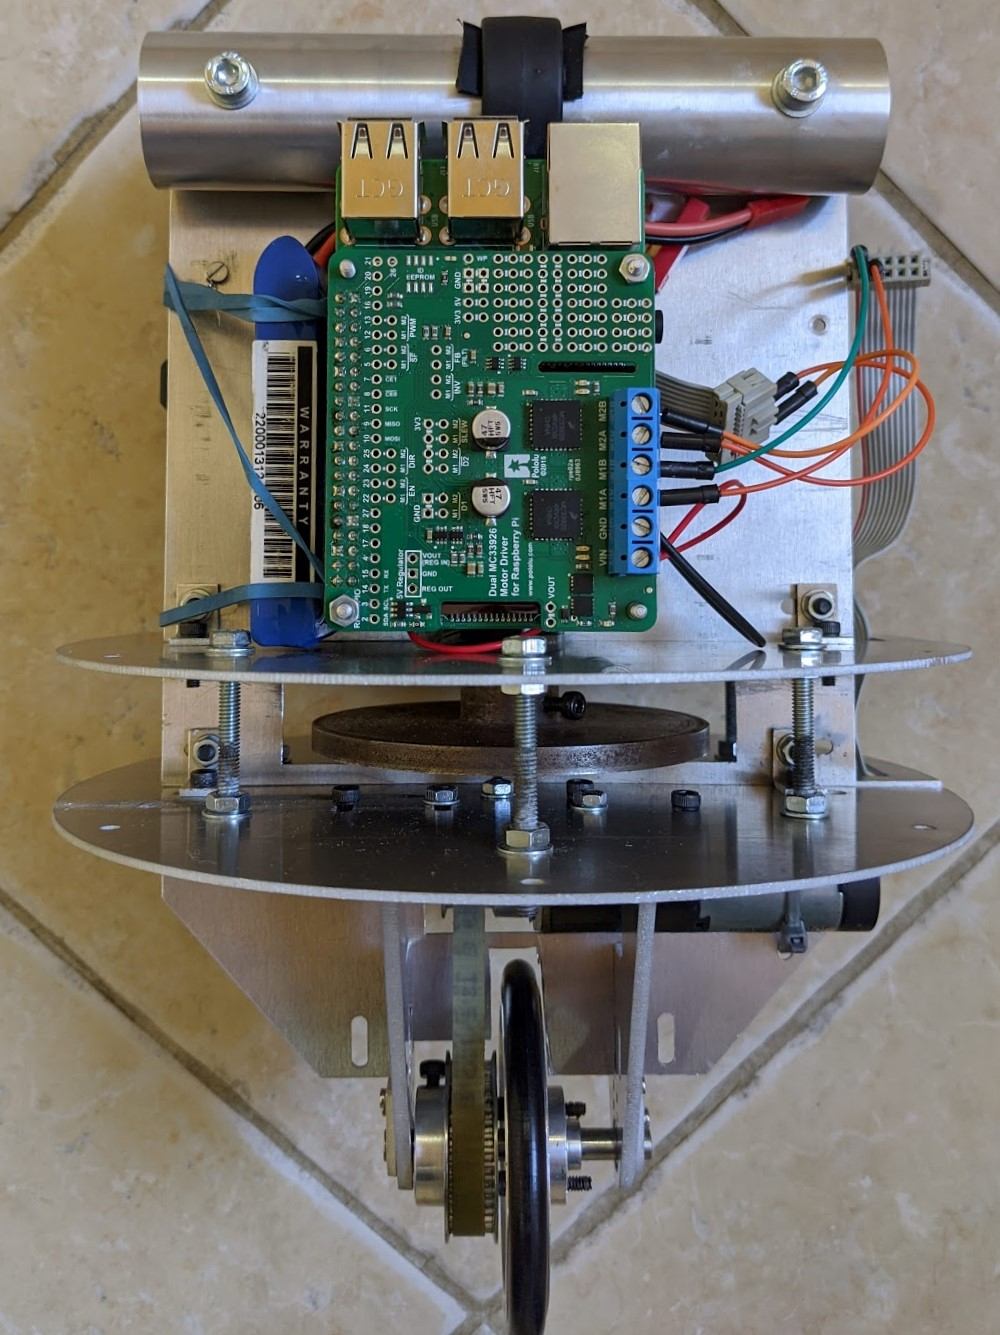
\includegraphics[width=\linewidth]{backnew}
    \caption{Back}
  \label{sub:backnew}
  \end{subfigure}
  \newline
  
  \begin{subfigure}[t]{0.325\textwidth}
    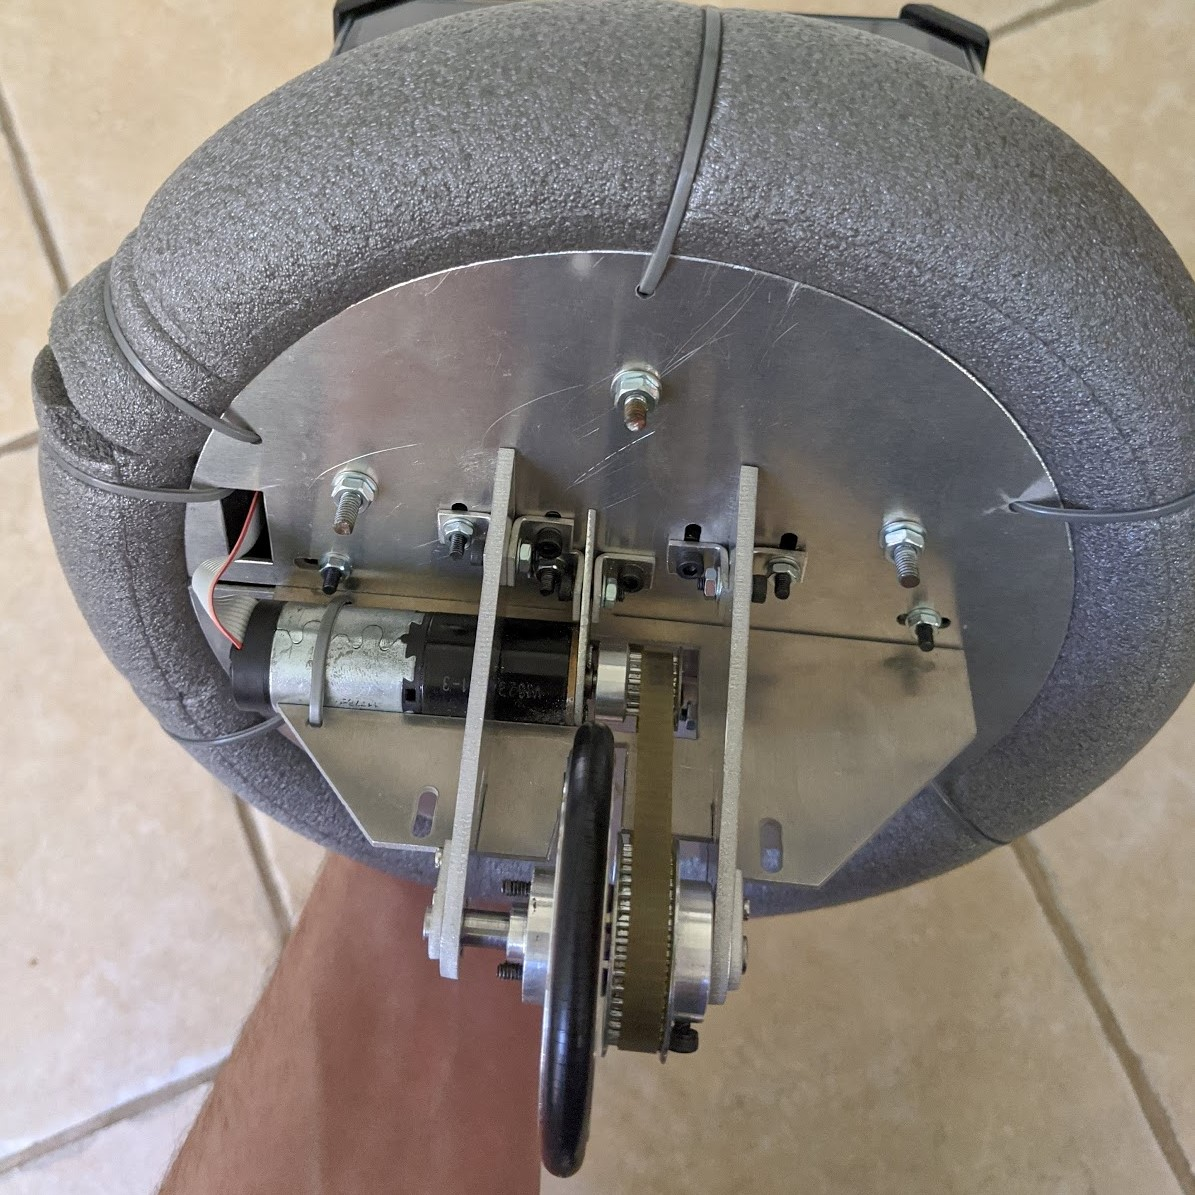
\includegraphics[width=\linewidth]{botnew}
    \caption{Bottom}
  \label{sub:botnew}
  \end{subfigure}
  \begin{subfigure}[t]{0.325\textwidth}
    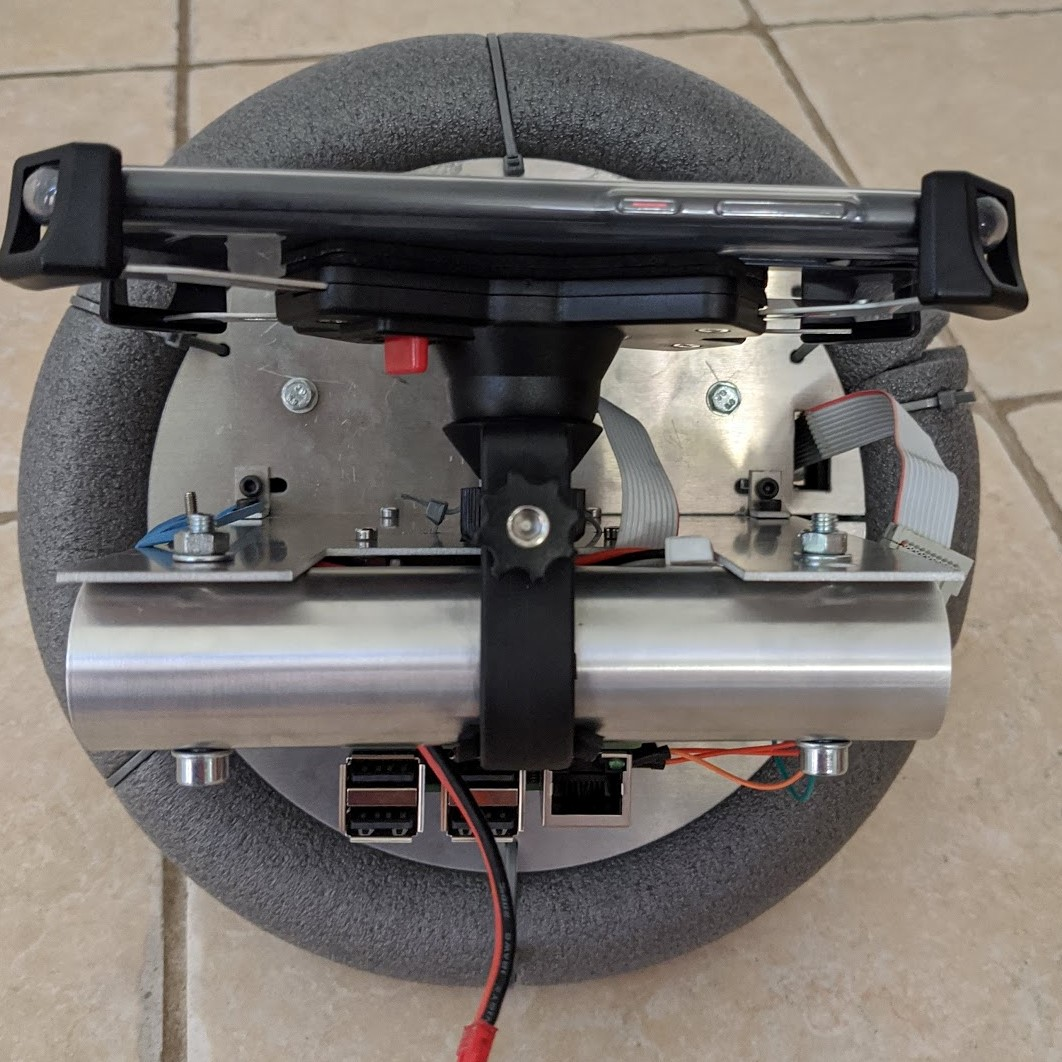
\includegraphics[width=\linewidth]{topnew}
    \caption{Top}
  \label{sub:topnew}
  \end{subfigure}
  
  \caption{New set-up of unicycle}
  \label{fig:new}
\end{figure*}

\section{Mechanical redesign}


\subsection{Changes}

%--------------------------------------
\subsection{Concerns}

%--------------------------------
\clearpage
\section{Results}
\subsection{Phone}
\subsubsection{Connection}
Previously the phone connected to the Matlab scrip on the computer using Matlab mobile and wifi. However, this feature has since been removed from Matlab mobile and delays caused by using wifi were believed to occur occasionally. This could introduce extra noise and incorrect state measurements decreasing learning ability.
\newline
HyperIMU \cite{ianovir} was used to replace Matlab mobile. This allowed connection using wifi and USB. The transmission protocol followed was UDP using the packet layout:

\begin{figure*}[t]
  \centering
  \begin{subfigure}[t]{0.325\textwidth}
    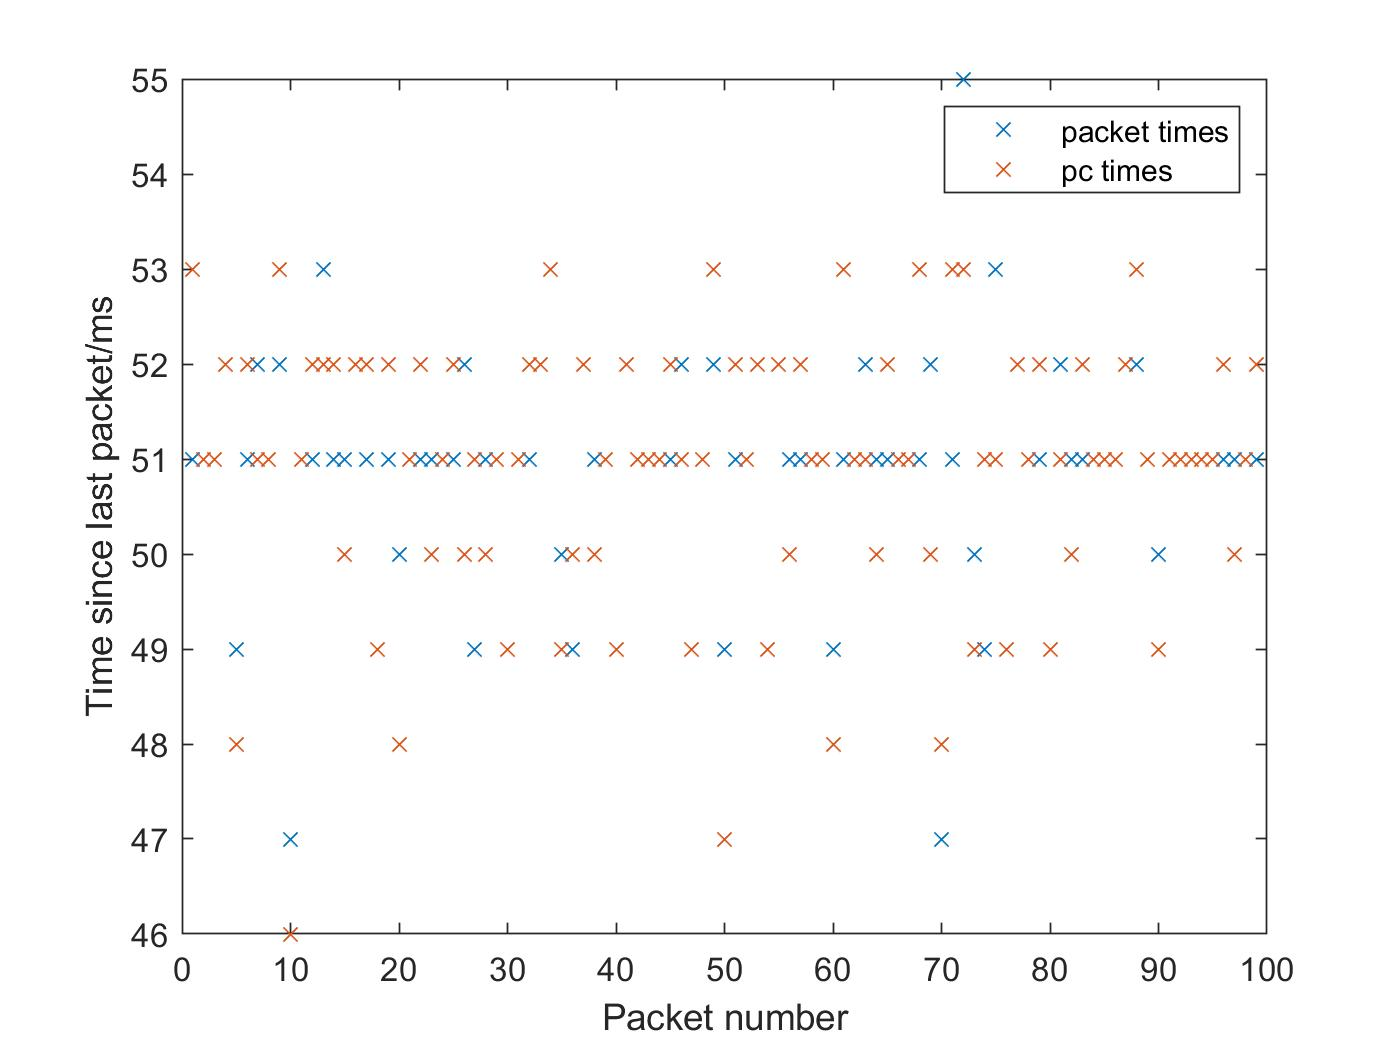
\includegraphics[width=\linewidth]{timestep}
   \caption{Time between measurements}
  \label{fig:ts}
  \end{subfigure}
  \begin{subfigure}[t]{0.325\textwidth}
    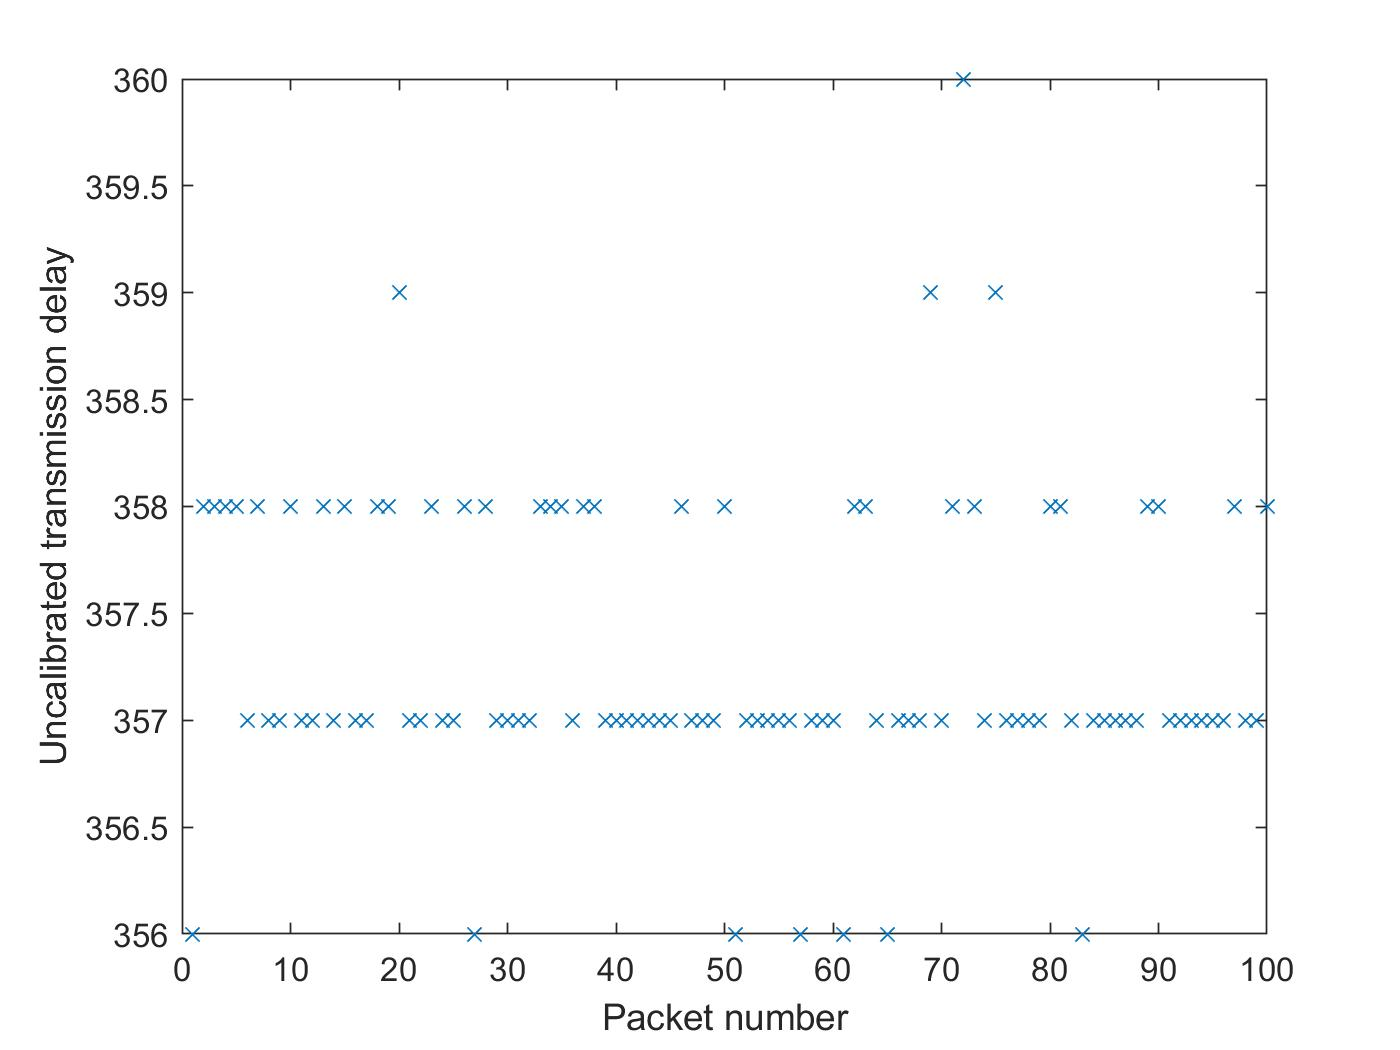
\includegraphics[width=\linewidth]{delay}
    \caption{Uncalibrated delay}
  \label{fig:td}
  \end{subfigure}
  \begin{subfigure}[t]{0.325\textwidth}
    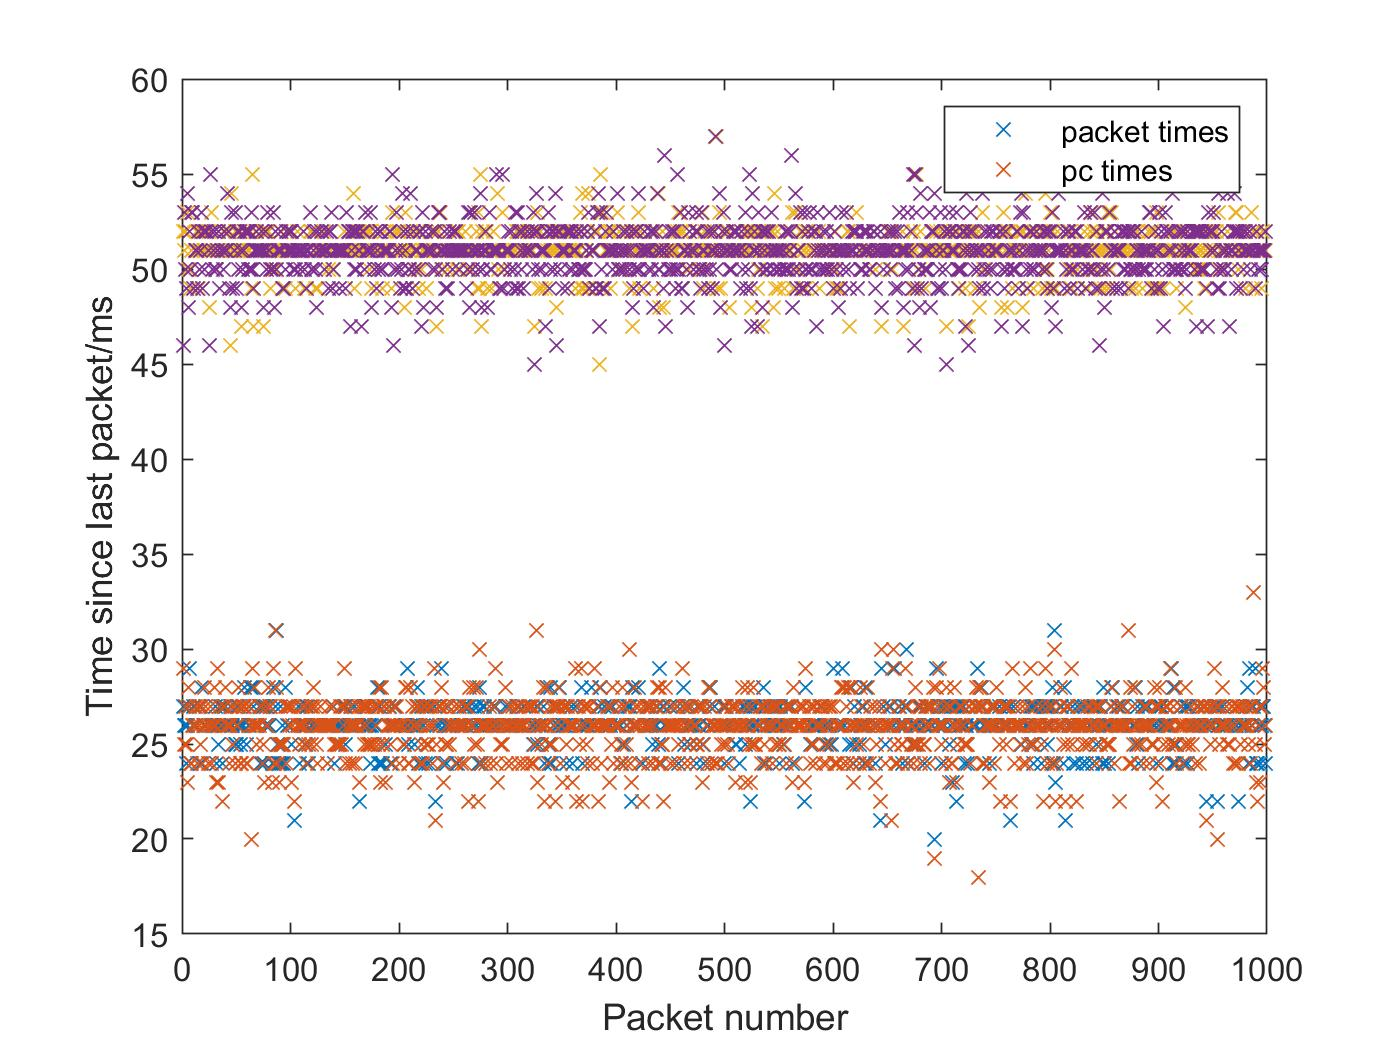
\includegraphics[width=\linewidth]{both}
    \caption{Different sampling times}
  \label{fig:ts2}
  \end{subfigure}
  \caption{Testing connecting by USB}
  \label{fig:usb}
\end{figure*}

\begin{align*}
[t, a_x, a_y ,a_z , \dot{\alpha}_x, \dot{\alpha}_y , \dot{\alpha}_z \#]
\end{align*}

UDP was chosen over serial communication protocols to take advantage of existing software and allow for wifi to easily be used again in the future if desired.

Tests were conducted to determine the reliability of this method. Figure \ref{fig:ts} shows the time between consecutive measurements on both the phone side and computer side. A mean of 50.89ms and standard deviation of 1.27ms was recorded over 1000 measurements. Variation is undesirable but this is small and times are known so won't prove problematic. A similar spread was observed at lower sampling times as shown in figure \ref{fig:ts2} where a 25ms sampling time resulted in a mean of 25.88ms and standard deviation of 1.38ms. This shows that this software is suitable if faster sampling times are required.
\newline
Due to different clocks on the computer and phone true transmission delay wasn't possible to measure. Figure \ref{fig:td} shows this uncalibrated delay. The majority of packets take one of two times to transmit with a few outliers taking $\pm$2ms. A low variation is desirable as it means actions can be applied for the correct length of time, as to not alter the trajectory away from the policy prediction.


\begin{figure}
  \centering
    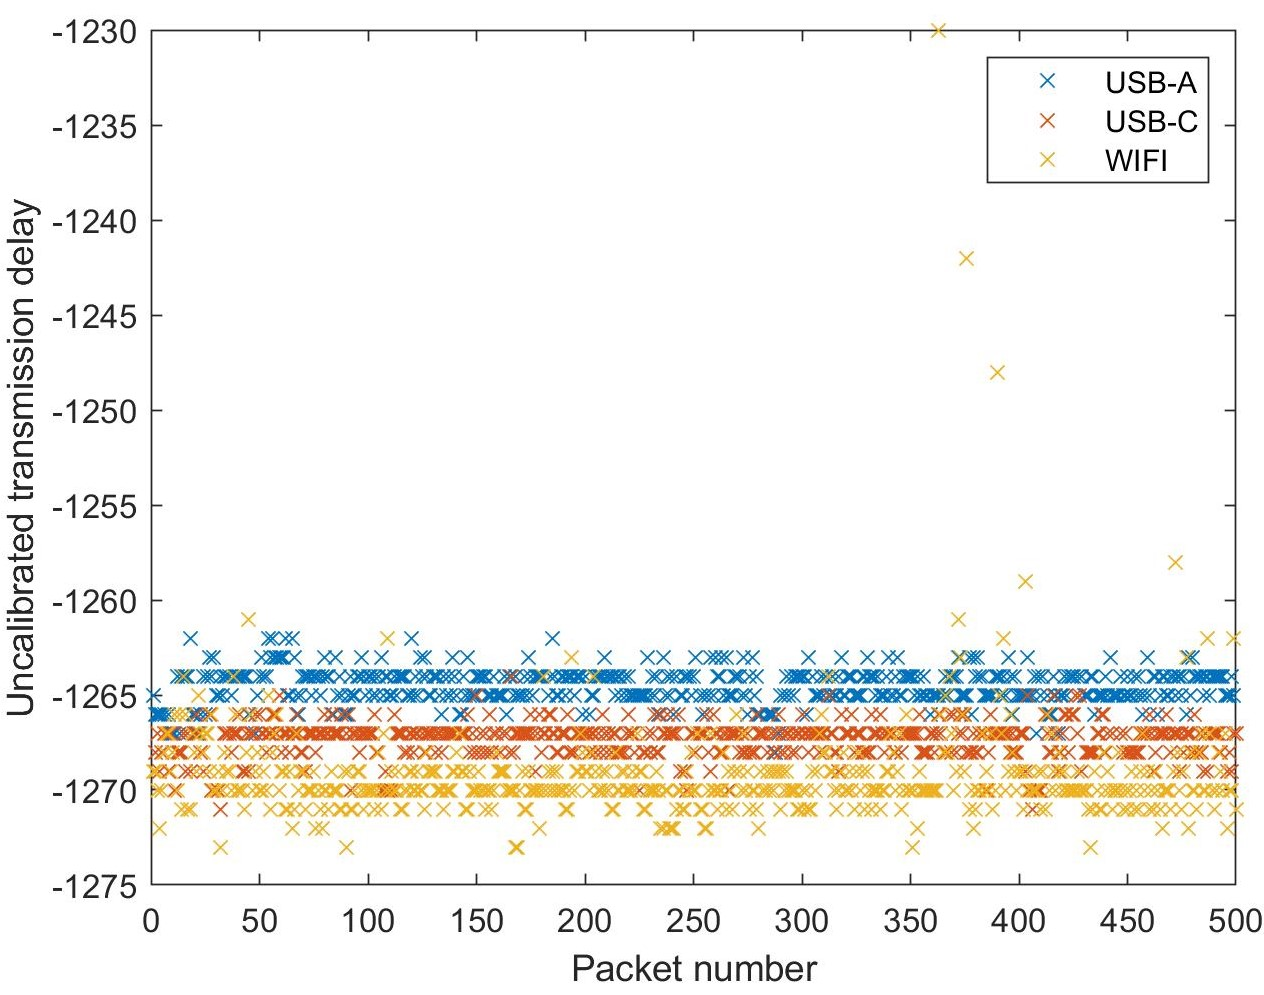
\includegraphics[width=\linewidth]{all3}
  \caption{Effect of changing transmission medium}
  \label{fig:med}
\end{figure}

\begin{table}[h]
\centering
\begin{tabular}{ c | c | c | c }
Test& USB-A & USB-C & WIFI\\ 
\midrule
1&0.99&1.05 &3.02\\
2&1.24& 1.26&1.25\\
3&1.10&1.02 &1.84\\
\end{tabular}
\caption{Transmission delay $\sigma$ in ms}
\label{table:td}
\end{table}
The delay over Three transmission mediums were compared in figure \ref{fig:med}. A smaller number on these graphs corresponds to a faster transmission. It was noticed that the difference between mediums was too large, this was explained when conducting the tests in different orders. The two clock times drifted apart after each test causing the exact delays to be incomparable, therefore flipping test order resulted in the opposite order to the figure. However, the variation in delay is what is most important when deciding method as this is what can cause unexpectedly long applied actions. Wifi showed some delays of nearly a whole time step in figure \ref{fig:med}. The standard deviation was calculated in Table \ref{table:td}. In test two the variation was almost identical amongst methods, but in the other tests wifi again showed greater variation. For this reason either USB connection is a better choice for use on the unicycle. The extra noise introduced by an extra cable effecting dynamics however may outweigh the transmission delay advantage and will need investigating. 
%------------------------------
\subsubsection{Orientation}
Imperfect starting positions in real rollouts can cause a constant offset in position throughout tests unless its determined at the start or learnt. Learning the offset is possible when training however due to the offline nature of rollouts can't be currently done on new runs. Measuring the initial orientation is therefore required, which also allows accurate uncertainty measurements ensuring predictions incorporate as much information as possible.
\begin{equation}
\begin{gathered}
\delta\textbf{a} = \textbf{a}_0 - R\hat{\textbf{a}} \\
\begin{bmatrix}
\theta \\
\psi_f \\
\end{bmatrix} = 
2 \begin{bmatrix}
tan^{-1} ( \frac{\delta\textbf{a}_x}{\sqrt{\delta\textbf{a}_y^2+\delta\textbf{a}_z^2}} )\\
-tan^{-1} ( \frac{\delta\textbf{a}_y}{\sqrt{\delta\textbf{a}_x^2+\delta\textbf{a}_z^2}} )\\
\end{bmatrix}
\label{eq:con}
\end{gathered}
\end{equation}
To calculate the initial orientation the roll and pitch angles between transformed accelerometer reading and $\textbf{a}_0 = [0,0,-1]^T$ needs to be determined. A transformation is required from the raw sensor acceleration to convert between phone and unicycle co-ordinates, this transformation being:

\begin{align*}
\textbf{a} = \begin{bmatrix}
0 & -1 & 0 \\
0 & 0 & -1\\
1 & 0 & 0 \\
\end{bmatrix}
\textbf{a}
\end{align*}



 The unicycle has only two angular DoF initially, this means that one angle can be set to 0. For this we choose yaw as this angle only depends on the starting position and is penalised when higher. The angles are measured for two seconds before initiating the rollout to estimate initial uncertainty.
\newline
Equation \ref{eq:con} calculates the initial euler orientation. This can then be easily converted to quaternion form with two quaternions rotations : (1 + 0\textbf{i}  + 0\textbf{j} + 0\textbf{k})$R_Y(\theta)R_X(\psi_f)$. Quaternions extend complex numbers to 4D and are required to accuracy keep track of repetitive rotations due to following the same mathematical rules. \cite{arsalan} Quaternion form is then used for all subsequent rotations calculated using gyroscope readings.
A rotation about axis (x,y,z) by $\alpha$ can be defined using the following unit quaternion.

\begin{gather}
\textbf{q} = cos(\frac{\alpha}{2}) + sin(\frac{\alpha}{2})(x\textbf{i} + y\textbf{j} + z\textbf{j}) \nonumber \\
\textbf{q}_{new} = \textbf{q}_{old} . \textbf{q} \nonumber
\end{gather}
  
\subsection{Rasberry Pi}
\subsubsection{Connection}

\begin{figure*}[t]
  \centering
  \begin{subfigure}[t]{0.325\textwidth}
    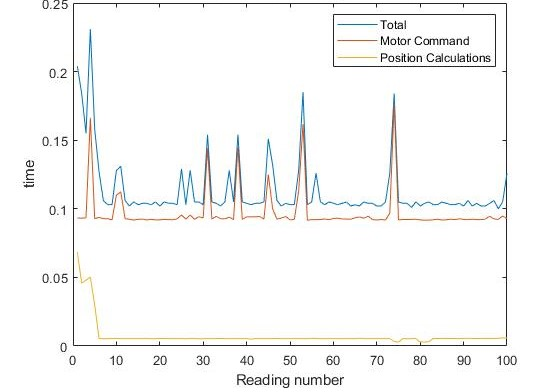
\includegraphics[width=\linewidth]{25ms_pi}
   \caption{25ms}
  \label{fig:pi25}
  \end{subfigure}
  \begin{subfigure}[t]{0.325\textwidth}
    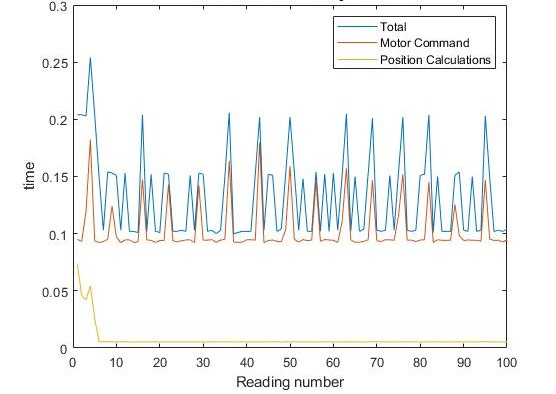
\includegraphics[width=\linewidth]{50ms_pi}
    \caption{50ms}
  \label{fig:pi50}
  \end{subfigure}
  \begin{subfigure}[t]{0.325\textwidth}
    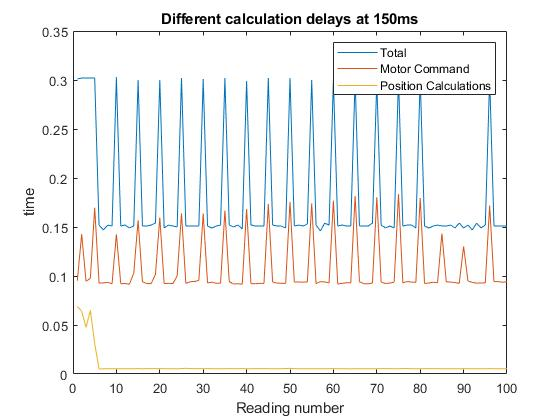
\includegraphics[width=\linewidth]{150ms_pi}
    \caption{150ms}
  \label{fig:pi150}
  \end{subfigure}
  \caption{Testing connecting from Matlab to Pi using Matlab system command}
  \label{fig:pi}
\end{figure*}

\begin{figure}
  \centering
    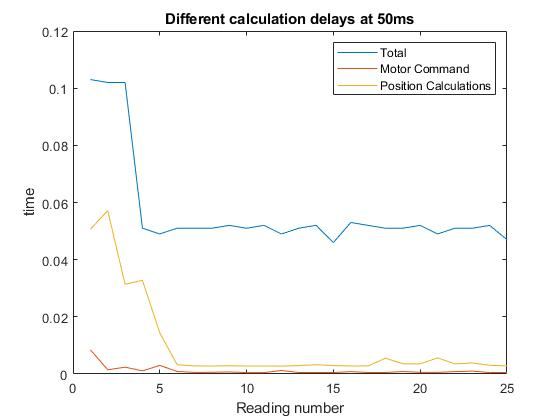
\includegraphics[width=\linewidth]{50ms_udp}
  \caption{Testing connection to Pi sending torques by UDP}
  \label{fig:piudp}
\end{figure} 
  
%----------------------------------
\subsection{Motor}
maybe something about calculating righting angles? and stiff


\subsection{Rollouts}
\onecolumn
\begin{figure*}[t]
  \centering
  \begin{subfigure}[t]{0.325\textwidth}
    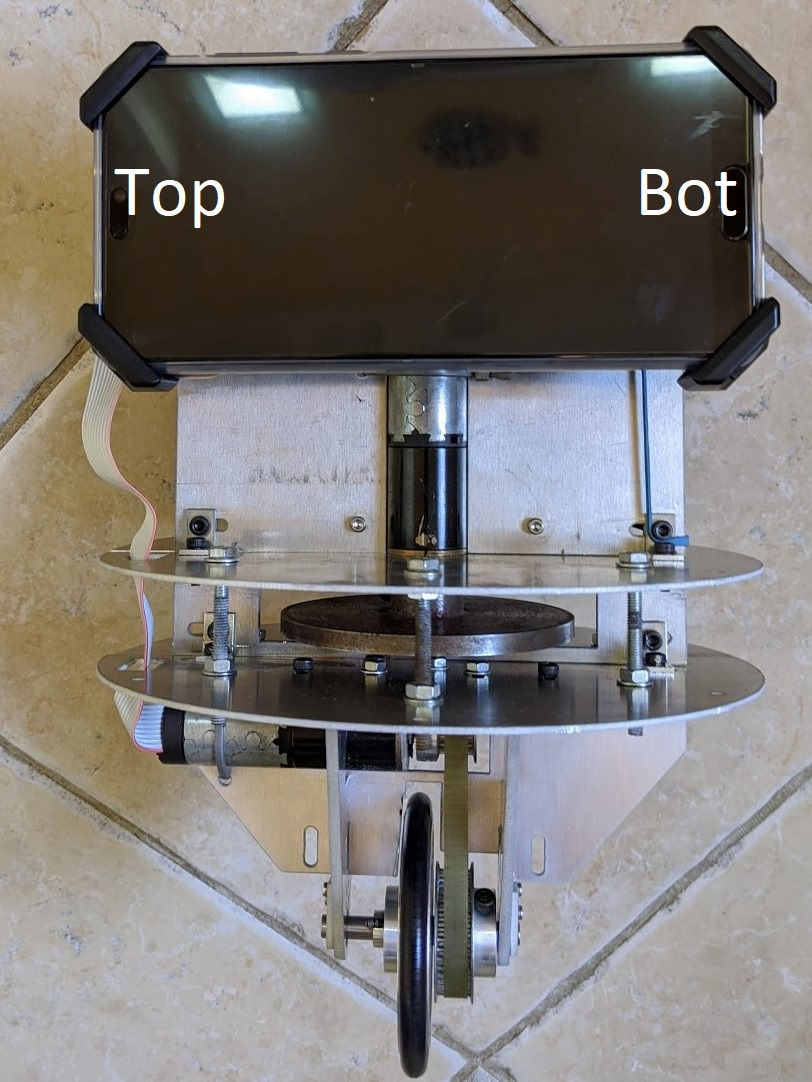
\includegraphics[width=\linewidth]{front_lab}
   \caption{Phone set-up}
  \label{fig:set_up}
  \end{subfigure}
  \begin{subfigure}[t]{0.325\textwidth}
    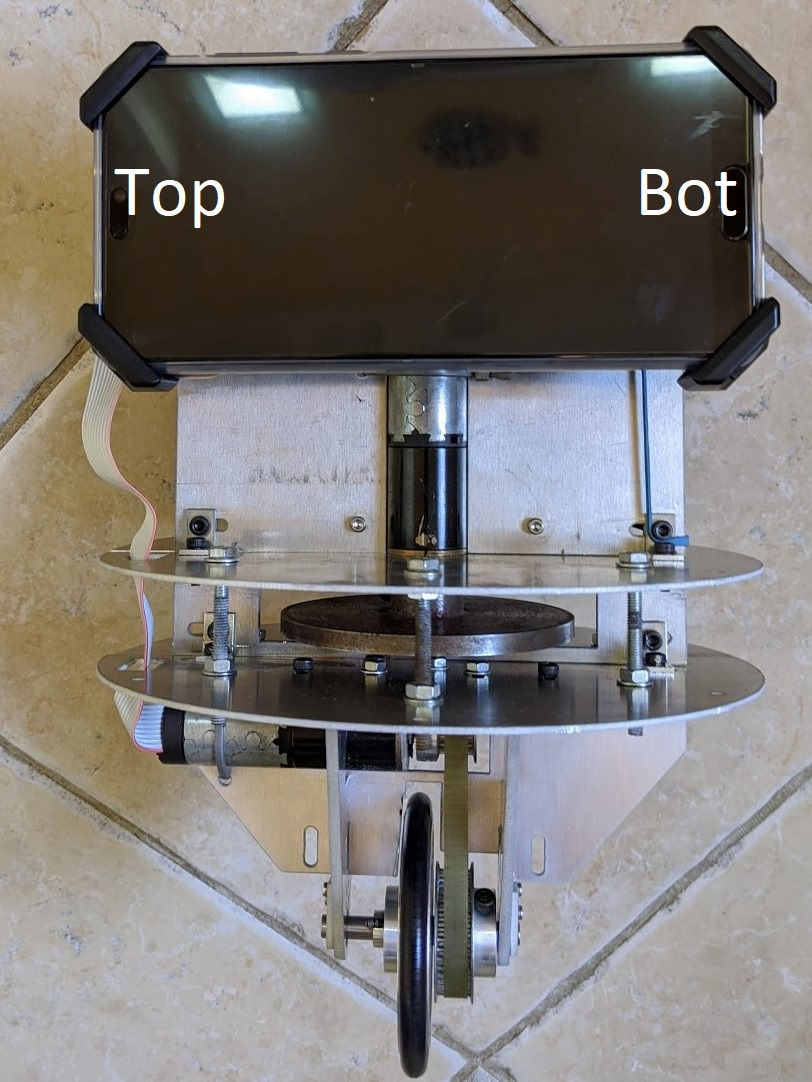
\includegraphics[width=\linewidth]{front_lab}
    \caption{HyperIMU settings}
  \label{fig:imuset}
  \end{subfigure}
  \begin{subfigure}[t]{0.325\textwidth}
    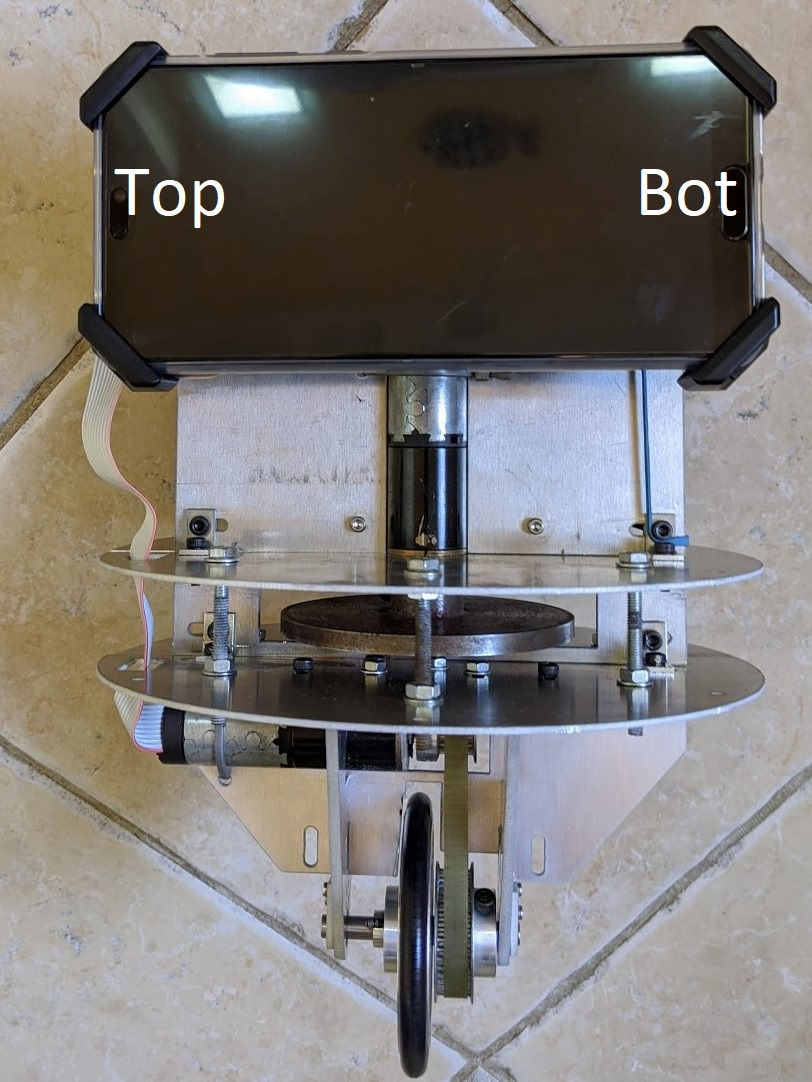
\includegraphics[width=\linewidth]{front_lab}
    \caption{Release position}
  \label{fig:unirel}
  \end{subfigure}
  \caption{Steps in set-up}
  \label{fig:set_up_steps}
\end{figure*}

\subsubsection{Test Procedure}

\textbf{Mechanical Set-Up}
\begin{itemize}
\item Attach phone as in figure \ref{fig:set_up} with the top of the phone facing to the left of the unicycle. Ensure the phone attachment is vertical and secure
\item Attach the Raspberry Pi using an Ethernet cable to the computer running Matlab
\item Connect phone to computer using a USB-A/C cable
\item Connect Raspberry Pi to 5V power source, and attach on board battery
\end{itemize}

\textbf{Software Set-Up}
\begin{itemize}
\item Turn on USB tethering in the phones settings (settings/network and internet/hotspot and tethering). This often works more reliably with the phone in aeroplane mode
\item Find the ipv4 address of the attached computer. on windows this is found by typing ipconfig into a command window
\item Open HyperIMU on the phone and go to settings and enter the ipv4 address, port 5555 and desired sample rate(this is often 1ms too slow) as figure \ref{fig:imuset}
\item Save these settings and click start logging from HyperIMU
\end{itemize}
\textbf{Rollouts}
\begin{itemize}
\item In an open flat space position the unicycle, run "doitreal.m" script from the connected computer
\item After initialisation a key press is required to initiate a rollout
\item Make sure that the unicycle is being held still and vertical at this point, holding onto the string improves repeatability and release smoothness as in figure \ref{fig:unirel}
\item The orientation is then measured for a few seconds before the motors start, at this point let go
\item After the unicycle has fallen the motors should terminate, and confirmation of a successful rollout is required in Matlab 
\item Policy optimisation and dynamics learning then ensues, the unicycle could be disconnected during this step
\item this is repeated until the desired rollouts are completed
\end{itemize}

\twocolumn
%------------------------------------------
\subsubsection{Functions}



%----------------------------
\subsubsection{Tests}

%---------------------------------
\subsection{Quadratic Controller}

%----------------------
\subsection{Additional Simulations}

%------------------------------------
\clearpage
\section{Conclusions}
\subsection{Progress}

%------------------------------
\subsection{Future Work}
After the further simulations has been performed and evaluated the following changes will be considered in the future:

\begin{itemize}
\item Redesign unicycle to allow for higher roll limit, different motors, greater modularity, robustness to falls and secure phone mounting.
\item Effect of independence between state variables on real rollouts.
\item Adjustments to cost function.
\end{itemize}


\subsection{Additional rollouts}


\subsection{Encoder}


\subsection{Exploration}


\subsection{Mass adjustment}

%----------------------------

%------------------------------------------------------------------------
\clearpage
\begin{thebibliography}{9}
\bibitem{pilco} 
M. P. Deisenroth and C. E. Rasmussen. ''PILCO: A Model-based and Data-Efficient Approach to Policy Search''.
2011. \url{http://www.icml-2011.org/papers/323_icmlpaper.pdf.}

\bibitem{original}
Mark Mellors, Andrew Lamb and J Maciejowski. 2005 \url{roboticunicycle.info} 

\bibitem{neil}
Neil D'Souza-Mathew. ''Balancing of a Robotic Unicycle''. MEng Thesis. CUED. 2008 \url{roboticunicycle.info/documents/MyFinalReport.pdf}

\bibitem{forster}
David Forster. ''Robotic Unicycle'' MEng Thesis. CUED. 2009

\bibitem{mchut}
Andrew McHutchon, ''Machine learning for Control''. MEng Thesis. CUED. 2010

\bibitem{roderigo}
Rodrigo Queiro. ''Machine Learning for Control''. MEng Thesis. CUED. 2011
\url{https://github.com/drigz/IIB-Project/blob/master/iibproject.pdf}

\bibitem{douglass}
Alan Douglass. ''Machine Learning for Control''. MEng Thesis. CUED. 2011

\bibitem{eric}
Eric Weiser. ''Robotic Unicycle'' . MEng Thesis. CUED. 2017

\bibitem{arsalan}
Arsalan Harris. ''Robotic Unicycle'' . MEng Thesis. CUED. 2019
 
 
\bibitem{ianovir} 
Ianovir: HyperIMU app 
\url{ianovir.com/works/mobile/hyperimu/}

\bibitem{other1}
mhexrobot. 2012. \url{https://edgetriggered.wordpress.com/category/unicycle-robot/}

\bibitem{other2}
G. Daoxiong, P. Qi, Z. Guoyu, and L. Xinghui, ''Lqr control for a self-balancing unicycle
robot on inclined plane''. 2012.

\bibitem{other3}
D. W. Vos and A. H. Von Flotow, ''Dynamics and nonlinear adaptive control of an
autonomous unicycle: Theory and experiment,'' in 29th IEEE Conference on Decision
and Control, pp. 182{187, IEEE, 1990.}

\bibitem{other4}
Matthew Davis. 2019 \url{https://www.mdavis.xyz/unicycle/}




\end{thebibliography}



%--------------------------------------------------
\clearpage
\section{Appendix}
\subsection{Risk Assessment Review}




%------------------------------------------------

%------------------------------------------------
\end{document}
